% Options for packages loaded elsewhere
\PassOptionsToPackage{unicode}{hyperref}
\PassOptionsToPackage{hyphens}{url}
%
\documentclass[
]{book}
\usepackage{amsmath,amssymb}
\usepackage{iftex}
\ifPDFTeX
  \usepackage[T1]{fontenc}
  \usepackage[utf8]{inputenc}
  \usepackage{textcomp} % provide euro and other symbols
\else % if luatex or xetex
  \usepackage{unicode-math} % this also loads fontspec
  \defaultfontfeatures{Scale=MatchLowercase}
  \defaultfontfeatures[\rmfamily]{Ligatures=TeX,Scale=1}
\fi
\usepackage{lmodern}
\ifPDFTeX\else
  % xetex/luatex font selection
\fi
% Use upquote if available, for straight quotes in verbatim environments
\IfFileExists{upquote.sty}{\usepackage{upquote}}{}
\IfFileExists{microtype.sty}{% use microtype if available
  \usepackage[]{microtype}
  \UseMicrotypeSet[protrusion]{basicmath} % disable protrusion for tt fonts
}{}
\makeatletter
\@ifundefined{KOMAClassName}{% if non-KOMA class
  \IfFileExists{parskip.sty}{%
    \usepackage{parskip}
  }{% else
    \setlength{\parindent}{0pt}
    \setlength{\parskip}{6pt plus 2pt minus 1pt}}
}{% if KOMA class
  \KOMAoptions{parskip=half}}
\makeatother
\usepackage{xcolor}
\usepackage{color}
\usepackage{fancyvrb}
\newcommand{\VerbBar}{|}
\newcommand{\VERB}{\Verb[commandchars=\\\{\}]}
\DefineVerbatimEnvironment{Highlighting}{Verbatim}{commandchars=\\\{\}}
% Add ',fontsize=\small' for more characters per line
\usepackage{framed}
\definecolor{shadecolor}{RGB}{248,248,248}
\newenvironment{Shaded}{\begin{snugshade}}{\end{snugshade}}
\newcommand{\AlertTok}[1]{\textcolor[rgb]{0.94,0.16,0.16}{#1}}
\newcommand{\AnnotationTok}[1]{\textcolor[rgb]{0.56,0.35,0.01}{\textbf{\textit{#1}}}}
\newcommand{\AttributeTok}[1]{\textcolor[rgb]{0.13,0.29,0.53}{#1}}
\newcommand{\BaseNTok}[1]{\textcolor[rgb]{0.00,0.00,0.81}{#1}}
\newcommand{\BuiltInTok}[1]{#1}
\newcommand{\CharTok}[1]{\textcolor[rgb]{0.31,0.60,0.02}{#1}}
\newcommand{\CommentTok}[1]{\textcolor[rgb]{0.56,0.35,0.01}{\textit{#1}}}
\newcommand{\CommentVarTok}[1]{\textcolor[rgb]{0.56,0.35,0.01}{\textbf{\textit{#1}}}}
\newcommand{\ConstantTok}[1]{\textcolor[rgb]{0.56,0.35,0.01}{#1}}
\newcommand{\ControlFlowTok}[1]{\textcolor[rgb]{0.13,0.29,0.53}{\textbf{#1}}}
\newcommand{\DataTypeTok}[1]{\textcolor[rgb]{0.13,0.29,0.53}{#1}}
\newcommand{\DecValTok}[1]{\textcolor[rgb]{0.00,0.00,0.81}{#1}}
\newcommand{\DocumentationTok}[1]{\textcolor[rgb]{0.56,0.35,0.01}{\textbf{\textit{#1}}}}
\newcommand{\ErrorTok}[1]{\textcolor[rgb]{0.64,0.00,0.00}{\textbf{#1}}}
\newcommand{\ExtensionTok}[1]{#1}
\newcommand{\FloatTok}[1]{\textcolor[rgb]{0.00,0.00,0.81}{#1}}
\newcommand{\FunctionTok}[1]{\textcolor[rgb]{0.13,0.29,0.53}{\textbf{#1}}}
\newcommand{\ImportTok}[1]{#1}
\newcommand{\InformationTok}[1]{\textcolor[rgb]{0.56,0.35,0.01}{\textbf{\textit{#1}}}}
\newcommand{\KeywordTok}[1]{\textcolor[rgb]{0.13,0.29,0.53}{\textbf{#1}}}
\newcommand{\NormalTok}[1]{#1}
\newcommand{\OperatorTok}[1]{\textcolor[rgb]{0.81,0.36,0.00}{\textbf{#1}}}
\newcommand{\OtherTok}[1]{\textcolor[rgb]{0.56,0.35,0.01}{#1}}
\newcommand{\PreprocessorTok}[1]{\textcolor[rgb]{0.56,0.35,0.01}{\textit{#1}}}
\newcommand{\RegionMarkerTok}[1]{#1}
\newcommand{\SpecialCharTok}[1]{\textcolor[rgb]{0.81,0.36,0.00}{\textbf{#1}}}
\newcommand{\SpecialStringTok}[1]{\textcolor[rgb]{0.31,0.60,0.02}{#1}}
\newcommand{\StringTok}[1]{\textcolor[rgb]{0.31,0.60,0.02}{#1}}
\newcommand{\VariableTok}[1]{\textcolor[rgb]{0.00,0.00,0.00}{#1}}
\newcommand{\VerbatimStringTok}[1]{\textcolor[rgb]{0.31,0.60,0.02}{#1}}
\newcommand{\WarningTok}[1]{\textcolor[rgb]{0.56,0.35,0.01}{\textbf{\textit{#1}}}}
\usepackage{longtable,booktabs,array}
\usepackage{calc} % for calculating minipage widths
% Correct order of tables after \paragraph or \subparagraph
\usepackage{etoolbox}
\makeatletter
\patchcmd\longtable{\par}{\if@noskipsec\mbox{}\fi\par}{}{}
\makeatother
% Allow footnotes in longtable head/foot
\IfFileExists{footnotehyper.sty}{\usepackage{footnotehyper}}{\usepackage{footnote}}
\makesavenoteenv{longtable}
\usepackage{graphicx}
\makeatletter
\newsavebox\pandoc@box
\newcommand*\pandocbounded[1]{% scales image to fit in text height/width
  \sbox\pandoc@box{#1}%
  \Gscale@div\@tempa{\textheight}{\dimexpr\ht\pandoc@box+\dp\pandoc@box\relax}%
  \Gscale@div\@tempb{\linewidth}{\wd\pandoc@box}%
  \ifdim\@tempb\p@<\@tempa\p@\let\@tempa\@tempb\fi% select the smaller of both
  \ifdim\@tempa\p@<\p@\scalebox{\@tempa}{\usebox\pandoc@box}%
  \else\usebox{\pandoc@box}%
  \fi%
}
% Set default figure placement to htbp
\def\fps@figure{htbp}
\makeatother
\setlength{\emergencystretch}{3em} % prevent overfull lines
\providecommand{\tightlist}{%
  \setlength{\itemsep}{0pt}\setlength{\parskip}{0pt}}
\setcounter{secnumdepth}{5}
\usepackage{booktabs}
\usepackage{amsthm}
\makeatletter
\def\thm@space@setup{%
  \thm@preskip=8pt plus 2pt minus 4pt
  \thm@postskip=\thm@preskip
}
\makeatother
\usepackage[]{natbib}
\bibliographystyle{plainnat}
\usepackage{bookmark}
\IfFileExists{xurl.sty}{\usepackage{xurl}}{} % add URL line breaks if available
\urlstyle{same}
\hypersetup{
  pdftitle={Calentamiento Global, Emisiones de Dióxido de Carbono y Crecimiento Económico: Una Perspectiva Regional y Económica},
  pdfauthor={Fabian Manrique},
  hidelinks,
  pdfcreator={LaTeX via pandoc}}

\title{Calentamiento Global, Emisiones de Dióxido de Carbono y Crecimiento Económico: Una Perspectiva Regional y Económica}
\author{Fabian Manrique}
\date{2026-04-24}

\begin{document}
\maketitle

{
\setcounter{tocdepth}{1}
\tableofcontents
}
\chapter{Resumen}\label{resumen}

El presente estudio tiene como objetivo principal analizar el paisaje global de las emisiones de gases de efecto invernadero, evaluando la interdependencia entre el desarrollo económico, la producción de emisiones de gases de efecto invernadero (GEI) y el incremento en la temperatura global media. Adicionalmente, La contribución científica de este trabajo reside en la integración de múltiples bases de datos climáticas y energéticas para diagnosticar las regiones del mundo que más han contribuido al total emitido a nivel global y analizar patrones económicos y de afectación futura para extraer conclusiones sobre el papel que juega y jugará cada región en este fenómeno.

Para la consecución de estos objetivos, se adopta un enfoque metodológico cuantitativo y comparativo fundamentado en datos históricos de temperatura y emisiones \citep{ref155}, así como información geopolítica de cada país. El resto del artículo se organiza de la siguiente manera. La segunda sección detalla el analisis exploratorio de los datos. La tercera sección presenta los resultados de la realización de pruebas de hipotesis para sustentar las conclusiones obtenidas en la segunda sección con evidencia numérica. Finalmente, la cuarta sección expone las conclusiones y recomendaciones obtenidas de nuestro análisis.

\chapter{Introducción}\label{introducciuxf3n}

La influencia antropogénica en el sistema climático global se ha consolidado como el principal motor del calentamiento contemporáneo \citep{ref1}. El incremento sostenido en las concentraciones de gases de efecto invernadero (GEI), derivados fundamentalmente de la combustión de combustibles fósiles, la producción de materiales industriales y los sistemas alimentarios, ha provocado un aumento inequívoco en la temperatura media de la superficie terrestre \citep{ref81}. Registros recientes indican que las anomalías térmicas globales han alcanzado aproximadamente 1.3°C en comparación con los niveles preindustriales, con variaciones regionales que superan los 5°C en zonas del Hemisferio Norte \citep{ref5}. Esta realidad climática exige una transformación profunda de los sistemas energéticos y productivos para mitigar impactos ambientales, económicos y sociales de carácter irreversible \citep{ref142}.

A pesar de la implementación de diversas políticas de mitigación a nivel internacional, las emisiones globales de dióxido de carbono (CO2) procedentes de fuentes fósiles aún no han alcanzado su pico máximo \citep{ref8}. El problema científico subyacente reside en la brecha crítica existente entre las políticas actuales, proyectadas para un calentamiento de 2.7°C hacia finales de siglo, y los objetivos del Acuerdo de París, que buscan limitar dicho aumento sustancialmente por debajo de los 2°C \citep{ref11}.

La literatura científica ha examinado extensamente la relación entre el suministro total de energía primaria y las trayectorias de emisión, observando que ambos indicadores han mostrado históricamente un comportamiento superpuesto \citep{ref107}. Trabajos previos destacan que, aunque el carbón representa una fracción minoritaria del suministro energético total, su combustión contribuye con el 45\% de las emisiones globales de CO2 \citep{ref112}. Se ha explorado el potencial del cambio tecnológico y de instrumentos económicos, como los impuestos al carbono y los sistemas de comercio de emisiones, para incentivar la descarbonización \citep{ref114}. No obstante, se identifican vacíos significativos en la efectividad de estos mecanismos, dado que la mayoría de las emisiones cubiertas por precios al carbono se sitúan por debajo de los niveles consistentes con las metas internacionales \citep{ref121}. Asimismo, aunque ciertos países han logrado desacoplar su crecimiento económico de las emisiones domésticas, este proceso no ocurre con la celeridad necesaria para estabilizar las concentraciones atmosféricas \citep{ref15}.

Además, persiste una marcada desigualdad en las contribuciones nacionales, donde los países con mayores niveles de riqueza emiten hasta 100 veces más por persona que las naciones con menores ingresos \citep{ref12}. Esta asimetría dificulta la adopción de una senda de desarrollo bajo en carbono que sea equitativa y global. Para las economías en vías de desarrollo, la implementación de medidas de reducción de la huella de carbono resulta costosa y se percibe como una desventaja influenciada por la dinámica política internacional. Estas naciones se ven forzadas a gestionar tensiones entre sus objetivos de crecimiento económico y las exigencias de reducción de emisiones de GEI, tales como la disminución en la quema de combustibles fósiles y su reemplazo por tecnologías de generación de energía sostenible \citep{ref2}. La transición tecnológica hacia fuentes limpias, aunque necesaria, impone barreras políticas y económicas significativas que los gobiernos deben sondear para garantizar que la mejora en los estándares de vida no se vea comprometida por el imperativo de la descarbonización acelerada \citep{ref3}.

\chapter{Objetivos}\label{objetivos}

\section{Objetivo General}\label{objetivo-general}

Evaluar la relación entre el aumento de temperatura global, las emisiciones de gases de efecto invernadero (específicamente el dioxido de carbono o CO\textsubscript{2}) y el desarrollo económico de cada país y región, para obtener conclusiones sobre la relación existente entre cada uno de estos fenómenos.

\begin{center}\rule{0.5\linewidth}{0.5pt}\end{center}

\section{Objetivos Específicos}\label{objetivos-especuxedficos}

\begin{enumerate}
\def\labelenumi{\arabic{enumi}.}
\tightlist
\item
  Analizar la correlación existente entre el incremento histórico de las emisiones de CO\textsubscript{2} y el incremento la temperatura media global.
\item
  Demostrar el impacto de los países con mayor crecimiento ecónomico en el total de las emisiones globales.
\item
  Explorar las diferencias en emisiones entre diferentes regiones geográficas del mundo y grupos económicos.
\item
  Evaluar el impacto que tendrá el calentamiento global en cada región y grupo económico, y comparar los niveles de afectación proyectados.
\end{enumerate}

\begin{center}\rule{0.5\linewidth}{0.5pt}\end{center}

\chapter{Metodología}\label{metodologuxeda}

\section{Origen de los Datos}\label{origen-de-los-datos}

Los datos utilizados provienen de diferentes fuentes, entre las cuales encontramos:
* El analisis realizado por el sitio Web `Our World in Data' \citep{ref1}.
* El repositorio de datos provisto por el `National Centers for Environmental Information (NCEI)' \citep{ref159}.
* El repositorio de datos `Climate Change Data' provisto por la agencia `World Bank' \citep{ref155}.

\section{Procesamiento de Datos}\label{procesamiento-de-datos}

Los datos de los diferentes conjuntos de datos fueron importados, transformados y procesados utilizando funciones específicas de R para la manipulación de conjuntos de datos.

Las librerías utilizadas fueron:

\begin{itemize}
\tightlist
\item
  ggplot2 \citep{R-ggplot2}
\item
  dplyr \citep{R-dplyr}
\item
  tidyr \citep{R-tidyr}
\item
  readr \citep{R-readr}
\item
  tidyverse \citep{R-tidyverse}
\item
  readxl \citep{R-readxl}
\item
  knitr \citep{R-knitr}.
\end{itemize}

\section{Importación de Librerías a usar}\label{importaciuxf3n-de-libreruxedas-a-usar}

\begin{Shaded}
\begin{Highlighting}[]
\FunctionTok{library}\NormalTok{(dplyr)}
\FunctionTok{library}\NormalTok{(ggplot2)}
\FunctionTok{library}\NormalTok{(tidyr)}
\FunctionTok{library}\NormalTok{(readr)}
\FunctionTok{library}\NormalTok{(tidyverse)}
\FunctionTok{library}\NormalTok{(readxl)}
\FunctionTok{library}\NormalTok{(knitr)}
\end{Highlighting}
\end{Shaded}

Mediante estas herramientas, se realizó una exploración inicial mediante gráficas para explorar correlaciones esperadas del entendimiento inicial del tema para obtener conclusiones. Posteriormente, se validarán estas conclusiones con pruebas estadísticas que las sustenten.

\begin{center}\rule{0.5\linewidth}{0.5pt}\end{center}

\chapter{Diccionario de Campos}\label{diccionario-de-campos}

\section{Importación de Datos}\label{importaciuxf3n-de-datos}

A continuación, realizamos una descripción breve de los campos de información encontrados en cada una de los datasets trabajados:

\begin{Shaded}
\begin{Highlighting}[]
\NormalTok{temperature\_data }\OtherTok{\textless{}{-}} \FunctionTok{read\_csv}\NormalTok{(}\StringTok{"./Data/data.csv"}\NormalTok{, }\AttributeTok{skip =} \DecValTok{3}\NormalTok{)}
\NormalTok{emissions\_data }\OtherTok{\textless{}{-}} \FunctionTok{read\_csv}\NormalTok{(}\StringTok{"./Data/annual{-}co2{-}emissions.csv"}\NormalTok{)}
\NormalTok{emissions\_per\_capita\_data }\OtherTok{\textless{}{-}} \FunctionTok{read\_csv}\NormalTok{(}\StringTok{"./Data/co2{-}emissions{-}per{-}capita.csv"}\NormalTok{)}
\NormalTok{climate\_change\_data }\OtherTok{\textless{}{-}} \FunctionTok{read\_excel}\NormalTok{(}\StringTok{"./Data/climate\_change.xlsx"}\NormalTok{, }\AttributeTok{sheet =} \StringTok{"Data"}\NormalTok{)}
\NormalTok{country\_data }\OtherTok{\textless{}{-}} \FunctionTok{read\_excel}\NormalTok{(}\StringTok{"./Data/climate\_change.xlsx"}\NormalTok{, }\AttributeTok{sheet =} \StringTok{"Country"}\NormalTok{)}
\NormalTok{series\_data }\OtherTok{\textless{}{-}} \FunctionTok{read\_excel}\NormalTok{(}\StringTok{"./Data/climate\_change.xlsx"}\NormalTok{, }\AttributeTok{sheet =} \StringTok{"Series"}\NormalTok{)}
\end{Highlighting}
\end{Shaded}

\section{\texorpdfstring{Dataset `Annual CO\textsubscript{2} Emissions'}{Dataset `Annual CO2 Emissions'}}\label{dataset-annual-co2-emissions}

Obtenido de \citep{ref1}, este dataset nos provee información histórica de las emisiones totales de cada entidad o país desde el año 1949.

\begin{longtable}[]{@{}
  >{\raggedright\arraybackslash}p{(\linewidth - 2\tabcolsep) * \real{0.4118}}
  >{\raggedright\arraybackslash}p{(\linewidth - 2\tabcolsep) * \real{0.5882}}@{}}
\toprule\noalign{}
\begin{minipage}[b]{\linewidth}\raggedright
Variable
\end{minipage} & \begin{minipage}[b]{\linewidth}\raggedright
Descripción
\end{minipage} \\
\midrule\noalign{}
\endhead
\bottomrule\noalign{}
\endlastfoot
Entity & País o agrupación de paises \\
Code & Código ISO-Alpha 3 (país) u OWID (agrupación) de la entidad \\
Year & Año de muestreo del dato \\
CO\textsubscript{2} emissions & Total emitido por la entidad en el año en cuestión en Toneladas \\
\end{longtable}

\begin{Shaded}
\begin{Highlighting}[]
\FunctionTok{str}\NormalTok{(emissions\_data) }\SpecialCharTok{\%\textgreater{}\%} \FunctionTok{kable}\NormalTok{()}
\end{Highlighting}
\end{Shaded}

\begin{verbatim}
## spc_tbl_ [29,384 x 4] (S3: spec_tbl_df/tbl_df/tbl/data.frame)
##  $ Entity              : chr [1:29384] "Afghanistan" "Afghanistan" "Afghanistan" "Afghanistan" ...
##  $ Code                : chr [1:29384] "AFG" "AFG" "AFG" "AFG" ...
##  $ Year                : num [1:29384] 1949 1950 1951 1952 1953 ...
##  $ Annual CO₂ emissions: num [1:29384] 14656 84272 91600 91600 106256 ...
##  - attr(*, "spec")=
##   .. cols(
##   ..   Entity = col_character(),
##   ..   Code = col_character(),
##   ..   Year = col_double(),
##   ..   `Annual CO₂ emissions` = col_double()
##   .. )
##  - attr(*, "problems")=<externalptr>
\end{verbatim}

\begin{tabular}{}
\hline

\hline
\end{tabular}

\section{\texorpdfstring{Dataset `CO\textsubscript{2} Emissions per Capita'}{Dataset `CO2 Emissions per Capita'}}\label{dataset-co2-emissions-per-capita}

Obtenido de \citep{ref1}, este dataset nos provee información histórica de las emisiones per capita de cada entidad o país desde el año 1949.

\begin{longtable}[]{@{}
  >{\raggedright\arraybackslash}p{(\linewidth - 2\tabcolsep) * \real{0.4118}}
  >{\raggedright\arraybackslash}p{(\linewidth - 2\tabcolsep) * \real{0.5882}}@{}}
\toprule\noalign{}
\begin{minipage}[b]{\linewidth}\raggedright
Variable
\end{minipage} & \begin{minipage}[b]{\linewidth}\raggedright
Descripción
\end{minipage} \\
\midrule\noalign{}
\endhead
\bottomrule\noalign{}
\endlastfoot
Entity & País o agrupación de paises \\
Code & Código ISO-Alpha 3 (país) u OWID (agrupación) de la entidad \\
Year & Year of the data \\
CO\textsubscript{2} emissions per capita & Total emitido por la entidad dividido por la población en el año en cuestión en Toneladas por persona \\
\end{longtable}

\begin{Shaded}
\begin{Highlighting}[]
\FunctionTok{str}\NormalTok{(emissions\_per\_capita\_data) }\SpecialCharTok{\%\textgreater{}\%} \FunctionTok{kable}\NormalTok{()}
\end{Highlighting}
\end{Shaded}

\begin{verbatim}
## spc_tbl_ [26,509 x 4] (S3: spec_tbl_df/tbl_df/tbl/data.frame)
##  $ Entity                  : chr [1:26509] "Afghanistan" "Afghanistan" "Afghanistan" "Afghanistan" ...
##  $ Code                    : chr [1:26509] "AFG" "AFG" "AFG" "AFG" ...
##  $ Year                    : num [1:26509] 1949 1950 1951 1952 1953 ...
##  $ CO₂ emissions per capita: num [1:26509] 0.00199 0.01084 0.01163 0.01147 0.01312 ...
##  - attr(*, "spec")=
##   .. cols(
##   ..   Entity = col_character(),
##   ..   Code = col_character(),
##   ..   Year = col_double(),
##   ..   `CO₂ emissions per capita` = col_double()
##   .. )
##  - attr(*, "problems")=<externalptr>
\end{verbatim}

\begin{tabular}{}
\hline

\hline
\end{tabular}

\section{Dataset `Global Land and Ocean 12-Month Period Average Temperature Anomalies'}\label{dataset-global-land-and-ocean-12-month-period-average-temperature-anomalies}

Obtenido de \citep{ref159}, este dataset nos provee información histórica de la temperatura anómala global promedio por mes desde diciembre de 1850.

\begin{longtable}[]{@{}
  >{\raggedright\arraybackslash}p{(\linewidth - 2\tabcolsep) * \real{0.4118}}
  >{\raggedright\arraybackslash}p{(\linewidth - 2\tabcolsep) * \real{0.5882}}@{}}
\toprule\noalign{}
\begin{minipage}[b]{\linewidth}\raggedright
Variable
\end{minipage} & \begin{minipage}[b]{\linewidth}\raggedright
Descripción
\end{minipage} \\
\midrule\noalign{}
\endhead
\bottomrule\noalign{}
\endlastfoot
Date & Mes de muestreo del dato en formato YYYYMM \\
Anomaly & Temperatura anómala, calculada como la diferencia entre la temperatura global promedio y la temperatura global promedio entre los años 1861 a 1890, en Celsius \\
\end{longtable}

\begin{Shaded}
\begin{Highlighting}[]
\FunctionTok{str}\NormalTok{(temperature\_data) }\SpecialCharTok{\%\textgreater{}\%} \FunctionTok{kable}\NormalTok{()}
\end{Highlighting}
\end{Shaded}

\begin{verbatim}
## spc_tbl_ [2,104 x 2] (S3: spec_tbl_df/tbl_df/tbl/data.frame)
##  $ Date   : num [1:2104] 185012 185101 185102 185103 185104 ...
##  $ Anomaly: num [1:2104] -0.15 -0.13 -0.13 -0.13 -0.12 -0.12 -0.12 -0.11 -0.09 -0.08 ...
##  - attr(*, "spec")=
##   .. cols(
##   ..   Date = col_double(),
##   ..   Anomaly = col_double()
##   .. )
##  - attr(*, "problems")=<externalptr>
\end{verbatim}

\begin{tabular}{}
\hline

\hline
\end{tabular}

\section{Dataset `Climate Change Data'}\label{dataset-climate-change-data}

Obtenido de \citep{ref155}, este dataset nos provee información histórica diferentes variables climaticas y geopolíticas de los países del mundo, desde el año 1990.

\begin{longtable}[]{@{}
  >{\raggedright\arraybackslash}p{(\linewidth - 2\tabcolsep) * \real{0.2500}}
  >{\raggedright\arraybackslash}p{(\linewidth - 2\tabcolsep) * \real{0.7500}}@{}}
\toprule\noalign{}
\begin{minipage}[b]{\linewidth}\raggedright
Variable
\end{minipage} & \begin{minipage}[b]{\linewidth}\raggedright
Descripción
\end{minipage} \\
\midrule\noalign{}
\endhead
\bottomrule\noalign{}
\endlastfoot
Country code & Código ISO-Alpha 3 (país) u OWID (agrupación) de la entidad \\
Country Name & Nombre de la agrupación o país \\
Series Code & Código de la variable muestreada \\
Series Name & Nombre de la variable muestreada \\
1990 - 2011 & Columnas que corresponden al año de muestreo. Para algunas variables, como proyecciones a futuro, solo se encuentra data en la columna 2011, correspondiente al valor de la proyección \\
\end{longtable}

\begin{Shaded}
\begin{Highlighting}[]
\FunctionTok{str}\NormalTok{(climate\_change\_data) }\SpecialCharTok{\%\textgreater{}\%} \FunctionTok{kable}\NormalTok{()}
\end{Highlighting}
\end{Shaded}

\begin{verbatim}
## tibble [13,512 x 28] (S3: tbl_df/tbl/data.frame)
##  $ Country code: chr [1:13512] "ABW" "ADO" "AFG" "AGO" ...
##  $ Country name: chr [1:13512] "Aruba" "Andorra" "Afghanistan" "Angola" ...
##  $ Series code : chr [1:13512] "AG.LND.EL5M.ZS" "AG.LND.EL5M.ZS" "AG.LND.EL5M.ZS" "AG.LND.EL5M.ZS" ...
##  $ Series name : chr [1:13512] "Land area below 5m (% of land area)" "Land area below 5m (% of land area)" "Land area below 5m (% of land area)" "Land area below 5m (% of land area)" ...
##  $ SCALE       : num [1:13512] 0 0 0 0 0 0 0 0 0 0 ...
##  $ Decimals    : num [1:13512] 1 1 1 1 1 1 1 1 1 1 ...
##  $ 1990        : chr [1:13512] "29.574809999999999" "0" "0" "0.20823459999999999" ...
##  $ 1991        : chr [1:13512] ".." ".." ".." ".." ...
##  $ 1992        : chr [1:13512] ".." ".." ".." ".." ...
##  $ 1993        : chr [1:13512] ".." ".." ".." ".." ...
##  $ 1994        : chr [1:13512] ".." ".." ".." ".." ...
##  $ 1995        : chr [1:13512] ".." ".." ".." ".." ...
##  $ 1996        : chr [1:13512] ".." ".." ".." ".." ...
##  $ 1997        : chr [1:13512] ".." ".." ".." ".." ...
##  $ 1998        : chr [1:13512] ".." ".." ".." ".." ...
##  $ 1999        : chr [1:13512] ".." ".." ".." ".." ...
##  $ 2000        : chr [1:13512] "29.574809999999999" "0" "0" "0.20823459999999999" ...
##  $ 2001        : chr [1:13512] ".." ".." ".." ".." ...
##  $ 2002        : chr [1:13512] ".." ".." ".." ".." ...
##  $ 2003        : chr [1:13512] ".." ".." ".." ".." ...
##  $ 2004        : chr [1:13512] ".." ".." ".." ".." ...
##  $ 2005        : chr [1:13512] ".." ".." ".." ".." ...
##  $ 2006        : chr [1:13512] ".." ".." ".." ".." ...
##  $ 2007        : chr [1:13512] ".." ".." ".." ".." ...
##  $ 2008        : chr [1:13512] ".." ".." ".." ".." ...
##  $ 2009        : chr [1:13512] ".." ".." ".." ".." ...
##  $ 2010        : chr [1:13512] ".." ".." ".." ".." ...
##  $ 2011        : chr [1:13512] ".." ".." ".." ".." ...
\end{verbatim}

\begin{tabular}{}
\hline

\hline
\end{tabular}

\begin{Shaded}
\begin{Highlighting}[]
\FunctionTok{str}\NormalTok{(country\_data) }\SpecialCharTok{\%\textgreater{}\%} \FunctionTok{kable}\NormalTok{()}
\end{Highlighting}
\end{Shaded}

\begin{verbatim}
## tibble [233 x 6] (S3: tbl_df/tbl/data.frame)
##  $ Country code    : chr [1:233] "EAP" "ECA" "EMU" "HIC" ...
##  $ Country name    : chr [1:233] "East Asia & Pacific" "Europe & Central Asia" "Euro area" "High income" ...
##  $ Capital city    : chr [1:233] ".." ".." ".." ".." ...
##  $ Region          : chr [1:233] "Aggregates" "Aggregates" "Aggregates" "Aggregates" ...
##  $ Income group    : chr [1:233] "Aggregates" "Aggregates" "Aggregates" "Aggregates" ...
##  $ Lending category: chr [1:233] "Aggregates" "Aggregates" "Aggregates" "Aggregates" ...
\end{verbatim}

\begin{tabular}{}
\hline

\hline
\end{tabular}

\begin{Shaded}
\begin{Highlighting}[]
\FunctionTok{str}\NormalTok{(series\_data) }\SpecialCharTok{\%\textgreater{}\%} \FunctionTok{kable}\NormalTok{()}
\end{Highlighting}
\end{Shaded}

\begin{verbatim}
## tibble [58 x 8] (S3: tbl_df/tbl/data.frame)
##  $ Series code: chr [1:58] "SP.POP.TOTL" "SP.POP.GROW" "NY.GDP.MKTP.CD" "NY.GNP.PCAP.CD" ...
##  $ Series name: chr [1:58] "Population" "Population growth (annual %)" "GDP ($)" "GNI per capita (Atlas $)" ...
##  $ Scale      : chr [1:58] "0" "0" "0" "0" ...
##  $ Decimals   : chr [1:58] "0" "1" "0" "0" ...
##  $ Order      : num [1:58] 1 2 3 4 5 6 7 8 9 10 ...
##  $ Topic      : chr [1:58] "Size of the economy" "Size of the economy" "Size of the economy" "Size of the economy" ...
##  $ Definition : chr [1:58] "Population includes all residents who are present regardless of legal status or citizenship except for refugees"| __truncated__ "Annual population growth rate for year t is the exponential rate of growth of midyear population from year t-1 "| __truncated__ "GDP is gross domestic product and measures the total output of goods and services for final use occurring withi"| __truncated__ "GNI per capita is the gross national income, converted to U.S. dollars using the World Bank Atlas method, divid"| __truncated__ ...
##  $ Source     : chr [1:58] "(1) United Nations Population Division. 2011. World Population Prospects: The 2010 Revision. New York, United N"| __truncated__ "Derived from total population. Population source: (1) United Nations Population Division. 2011. World Populatio"| __truncated__ "World Bank national accounts data, and OECD National Accounts data files." "World Bank national accounts data, and OECD National Accounts data files." ...
\end{verbatim}

\begin{tabular}{}
\hline

\hline
\end{tabular}

\begin{itemize}
\tightlist
\item
  Variables utilizadas:
\end{itemize}

\begin{longtable}[]{@{}
  >{\raggedright\arraybackslash}p{(\linewidth - 4\tabcolsep) * \real{0.1772}}
  >{\raggedright\arraybackslash}p{(\linewidth - 4\tabcolsep) * \real{0.1772}}
  >{\raggedright\arraybackslash}p{(\linewidth - 4\tabcolsep) * \real{0.6456}}@{}}
\toprule\noalign{}
\begin{minipage}[b]{\linewidth}\raggedright
Variable
\end{minipage} & \begin{minipage}[b]{\linewidth}\raggedright
Codigo
\end{minipage} & \begin{minipage}[b]{\linewidth}\raggedright
Descripción
\end{minipage} \\
\midrule\noalign{}
\endhead
\bottomrule\noalign{}
\endlastfoot
Population & SP.POP.TOTL & Población de la entidad \\
GDP & NY.GDP.MKTP.CD & PIB total en doláres de la entidad \\
Projected annual temperature change (2045-2065, Celsius) & EN.CLC.PCAT.C & Cambio de temperatura proyectado para el periodo 2045 a 2065 en Celsius \\
Projected annual precipitation change (2045-2065, mm) & EN.CLC.PCPT.MM & Cambio en total de precipitaciones proyectado para el periodo de 2045 a 2065, en mm \\
\end{longtable}

\chapter{Análisis Exploratorio de Datos}\label{anuxe1lisis-exploratorio-de-datos}

\section{Procesamiento de Datos}\label{procesamiento-de-datos-1}

Debido al uso de datos de diferente origen, es necesario limpiar, organizar y fusionar los conjuntos de datos usados. Esto inclye procesamiento de algunas columnas como la columna Date del dataset de temperaturas anómalas e identificar agrupaciones de países y variables de interes.

\begin{Shaded}
\begin{Highlighting}[]
\NormalTok{temperature\_data}\SpecialCharTok{$}\NormalTok{year }\OtherTok{=} \FunctionTok{as.integer}\NormalTok{(}\FunctionTok{substr}\NormalTok{(temperature\_data}\SpecialCharTok{$}\NormalTok{Date, }\DecValTok{1}\NormalTok{, }\DecValTok{4}\NormalTok{))}
\NormalTok{temperature\_data}\SpecialCharTok{$}\NormalTok{month }\OtherTok{=} \FunctionTok{as.integer}\NormalTok{(}\FunctionTok{substr}\NormalTok{(temperature\_data}\SpecialCharTok{$}\NormalTok{Date, }\DecValTok{5}\NormalTok{, }\DecValTok{6}\NormalTok{))}

\NormalTok{gdp\_data }\OtherTok{\textless{}{-}}\NormalTok{ climate\_change\_data }\SpecialCharTok{\%\textgreater{}\%}  
  \FunctionTok{filter}\NormalTok{(}\StringTok{\textasciigrave{}}\AttributeTok{Series code}\StringTok{\textasciigrave{}} \SpecialCharTok{\%in\%} \FunctionTok{c}\NormalTok{(}\StringTok{"NY.GDP.MKTP.CD"}\NormalTok{, }\StringTok{"SP.POP.TOTL"}\NormalTok{)) }\SpecialCharTok{\%\textgreater{}\%} 
  \FunctionTok{pivot\_longer}\NormalTok{(}
    \AttributeTok{cols =}\NormalTok{ (}\FunctionTok{ncol}\NormalTok{(.)}\SpecialCharTok{{-}}\DecValTok{21}\NormalTok{)}\SpecialCharTok{:}\FunctionTok{ncol}\NormalTok{(.),}
    \AttributeTok{names\_to =} \StringTok{"Year"}\NormalTok{,}
    \AttributeTok{values\_to =} \StringTok{"Value"}
\NormalTok{  ) }\SpecialCharTok{\%\textgreater{}\%} 
  \FunctionTok{select}\NormalTok{(}\SpecialCharTok{{-}}\StringTok{\textasciigrave{}}\AttributeTok{Series code}\StringTok{\textasciigrave{}}\NormalTok{, }\SpecialCharTok{{-}}\NormalTok{SCALE, }\SpecialCharTok{{-}}\NormalTok{Decimals) }\SpecialCharTok{\%\textgreater{}\%} 
  \FunctionTok{pivot\_wider}\NormalTok{(}
    \AttributeTok{names\_from =} \StringTok{\textasciigrave{}}\AttributeTok{Series name}\StringTok{\textasciigrave{}}\NormalTok{,}
    \AttributeTok{values\_from =}\NormalTok{ Value}
\NormalTok{  ) }\SpecialCharTok{\%\textgreater{}\%} 
  \FunctionTok{mutate}\NormalTok{(}\StringTok{\textasciigrave{}}\AttributeTok{GDP ($)}\StringTok{\textasciigrave{}} \OtherTok{=} \FunctionTok{as.numeric}\NormalTok{(}\StringTok{\textasciigrave{}}\AttributeTok{GDP ($)}\StringTok{\textasciigrave{}}\NormalTok{)) }\SpecialCharTok{\%\textgreater{}\%} 
  \FunctionTok{mutate}\NormalTok{(}\StringTok{\textasciigrave{}}\AttributeTok{Population}\StringTok{\textasciigrave{}} \OtherTok{=} \FunctionTok{as.numeric}\NormalTok{(}\StringTok{\textasciigrave{}}\AttributeTok{Population}\StringTok{\textasciigrave{}}\NormalTok{)) }\SpecialCharTok{\%\textgreater{}\%} 
  \FunctionTok{mutate}\NormalTok{(}\StringTok{\textasciigrave{}}\AttributeTok{Year}\StringTok{\textasciigrave{}} \OtherTok{=} \FunctionTok{as.integer}\NormalTok{(}\StringTok{\textasciigrave{}}\AttributeTok{Year}\StringTok{\textasciigrave{}}\NormalTok{)) }\SpecialCharTok{\%\textgreater{}\%} 
  \FunctionTok{mutate}\NormalTok{(}\AttributeTok{gdp\_per\_capita =} \StringTok{\textasciigrave{}}\AttributeTok{GDP ($)}\StringTok{\textasciigrave{}}\SpecialCharTok{/}\NormalTok{Population)}

\NormalTok{yearly\_average }\OtherTok{\textless{}{-}}\NormalTok{ temperature\_data }\SpecialCharTok{\%\textgreater{}\%} \FunctionTok{summarise}\NormalTok{(}\AttributeTok{mean\_temperature =} \FunctionTok{mean}\NormalTok{(Anomaly), }\AttributeTok{.by=}\NormalTok{year)}


\NormalTok{emissions\_data}\SpecialCharTok{$}\NormalTok{Code }\OtherTok{\textless{}{-}} \FunctionTok{as.factor}\NormalTok{(emissions\_data}\SpecialCharTok{$}\NormalTok{Code) }

\NormalTok{emissions\_data }\SpecialCharTok{\%\textgreater{}\%}
  \FunctionTok{distinct}\NormalTok{(Entity, Code) }\OtherTok{{-}\textgreater{}}\NormalTok{ distinct\_codes}

\NormalTok{gdp\_data }\SpecialCharTok{\%\textgreater{}\%} 
  \FunctionTok{inner\_join}\NormalTok{(emissions\_data, }\AttributeTok{by=}\FunctionTok{c}\NormalTok{(}\StringTok{"Year"}\NormalTok{, }\StringTok{"Country code"} \OtherTok{=} \StringTok{"Code"}\NormalTok{)) }\SpecialCharTok{\%\textgreater{}\%}
  \FunctionTok{drop\_na}\NormalTok{() }\SpecialCharTok{\%\textgreater{}\%} \FunctionTok{select}\NormalTok{(}\StringTok{\textasciigrave{}}\AttributeTok{Country code}\StringTok{\textasciigrave{}}\NormalTok{, }\StringTok{"Country"} \OtherTok{=} \StringTok{\textasciigrave{}}\AttributeTok{Country name}\StringTok{\textasciigrave{}}\NormalTok{, Year, }\StringTok{"GDP"} \OtherTok{=} \StringTok{\textasciigrave{}}\AttributeTok{GDP ($)}\StringTok{\textasciigrave{}}\NormalTok{, Population, }\StringTok{"GDP per Capita"}\OtherTok{=}\NormalTok{gdp\_per\_capita, }\StringTok{"Annual CO2 emissions"} \OtherTok{=} \StringTok{\textasciigrave{}}\AttributeTok{Annual CO₂ emissions}\StringTok{\textasciigrave{}}\NormalTok{) }\OtherTok{{-}\textgreater{}}\NormalTok{ gdp\_joined\_data}

\NormalTok{distinct\_codes }\SpecialCharTok{\%\textgreater{}\%} \FunctionTok{filter}\NormalTok{(}\FunctionTok{startsWith}\NormalTok{(}\FunctionTok{as.character}\NormalTok{(Code), }\StringTok{"OWID"}\NormalTok{) }\SpecialCharTok{|} \FunctionTok{is.na}\NormalTok{(Code)) }\OtherTok{{-}\textgreater{}}\NormalTok{ special\_categories}

\NormalTok{income\_codes }\OtherTok{\textless{}{-}}\NormalTok{ special\_categories }\SpecialCharTok{\%\textgreater{}\%} \FunctionTok{filter}\NormalTok{(}\FunctionTok{grepl}\NormalTok{(}\StringTok{"income"}\NormalTok{, }\FunctionTok{as.character}\NormalTok{(Entity), }\AttributeTok{ignore.case =} \ConstantTok{TRUE}\NormalTok{)) }

\NormalTok{income\_data }\OtherTok{\textless{}{-}}\NormalTok{ emissions\_data }\SpecialCharTok{\%\textgreater{}\%} \FunctionTok{filter}\NormalTok{(Code }\SpecialCharTok{\%in\%}\NormalTok{ income\_codes}\SpecialCharTok{$}\NormalTok{Code) }\SpecialCharTok{\%\textgreater{}\%} \FunctionTok{left\_join}\NormalTok{(emissions\_per\_capita\_data, }\AttributeTok{by =} \FunctionTok{c}\NormalTok{(}\StringTok{"Code"}\NormalTok{, }\StringTok{"Entity"}\NormalTok{, }\StringTok{"Year"}\NormalTok{))}

\FunctionTok{colnames}\NormalTok{(income\_data) }\OtherTok{\textless{}{-}} \FunctionTok{c}\NormalTok{(}\StringTok{"Entity"}\NormalTok{, }\StringTok{"Code"}\NormalTok{, }\StringTok{"Year"}\NormalTok{, }\StringTok{"CO2 emissions"}\NormalTok{, }\StringTok{"CO2 per capita"}\NormalTok{)}
\end{Highlighting}
\end{Shaded}

\section{\texorpdfstring{Relación histórica entre emisiones de CO\textsubscript{2} y aumento de la temperatura promedio global.}{Relación histórica entre emisiones de CO2 y aumento de la temperatura promedio global.}}\label{relaciuxf3n-histuxf3rica-entre-emisiones-de-co2-y-aumento-de-la-temperatura-promedio-global.}

A continuación, se presenta una gráfica \ref{fig:1} con el comportamiento histórico de las emisiones totales de CO2 a través de los años. Adicionalmente, se incluye en el mismo gráfico el comportamiento anual de la temperatura anómala durante el mismo periodo de tiempo. El análisis de la gráfica revela una clara correlación positiva y estrecha entre las emisiones totales de CO2 y el incremento de la temperatura global, mostrando trayectorias que aparecen prácticamente superpuestas a lo largo del registro histórico.

Se observa un patrón de crecimiento acelerado en ambas variables durante los últimos cincuenta años, periodo en el cual han aumentado rápidamente sin alcanzar aún su pico máximo. Esta tendencia ascendente ha impulsado la temperatura media global hasta alcanzar anomalías de aproximadamente 1.3°C en comparación con los niveles preindustriales.

Diferencias resaltables entre ambas curvas pueden ser que mientras que la curva de emisiones totales presenta un comportamiento sostenido y suave, la temperatura manifiesta una mayor variabilidad natural año tras año, aunque sigue fielmente la tendencia de crecimiento exponencial.

En la figura \ref{fig:2}, se puede visualizar directamente la correlación entre ambas variables. Se evidencia una clara relación lineal positiva que complementa lo prensentado en la primera gráfica.

\begin{Shaded}
\begin{Highlighting}[]
\NormalTok{world\_co2 }\OtherTok{\textless{}{-}}\NormalTok{ emissions\_data }\SpecialCharTok{\%\textgreater{}\%} \FunctionTok{filter}\NormalTok{(Code }\SpecialCharTok{==} \StringTok{"OWID\_WRL"}\NormalTok{)}
\NormalTok{world\_per\_capita }\OtherTok{\textless{}{-}}\NormalTok{ emissions\_per\_capita\_data }\SpecialCharTok{\%\textgreater{}\%} \FunctionTok{filter}\NormalTok{(Code }\SpecialCharTok{==} \StringTok{"OWID\_WRL"}\NormalTok{)}

\NormalTok{yearly\_data }\OtherTok{\textless{}{-}}\NormalTok{ yearly\_average }\SpecialCharTok{\%\textgreater{}\%} 
  \FunctionTok{left\_join}\NormalTok{(world\_co2, }\AttributeTok{by =} \FunctionTok{c}\NormalTok{(}\StringTok{"year"} \OtherTok{=} \StringTok{"Year"}\NormalTok{)) }\SpecialCharTok{\%\textgreater{}\%} 
  \FunctionTok{select}\NormalTok{(}\SpecialCharTok{{-}}\NormalTok{Entity, }\SpecialCharTok{{-}}\NormalTok{ Code) }\SpecialCharTok{\%\textgreater{}\%}
  \FunctionTok{left\_join}\NormalTok{(world\_per\_capita, }\AttributeTok{by =} \FunctionTok{c}\NormalTok{(}\StringTok{"year"} \OtherTok{=} \StringTok{"Year"}\NormalTok{)) }\SpecialCharTok{\%\textgreater{}\%} 
  \FunctionTok{select}\NormalTok{(}\SpecialCharTok{{-}}\NormalTok{Entity, }\SpecialCharTok{{-}}\NormalTok{ Code)}
  
  
\FunctionTok{colnames}\NormalTok{(yearly\_data) }\OtherTok{\textless{}{-}} \FunctionTok{c}\NormalTok{(}\StringTok{"year"}\NormalTok{, }\StringTok{"mean\_temperature\_anomaly"}\NormalTok{, }\StringTok{"CO2\_emissions"}\NormalTok{, }\StringTok{"CO2 per capita"}\NormalTok{)}

\NormalTok{scale\_factor }\OtherTok{\textless{}{-}} \FunctionTok{max}\NormalTok{(yearly\_data}\SpecialCharTok{$}\NormalTok{CO2\_emissions, }\AttributeTok{na.rm =} \ConstantTok{TRUE}\NormalTok{) }\SpecialCharTok{/} \FunctionTok{max}\NormalTok{(yearly\_data}\SpecialCharTok{$}\NormalTok{mean\_temperature\_anomaly, }\AttributeTok{na.rm =} \ConstantTok{TRUE}\NormalTok{)}
\end{Highlighting}
\end{Shaded}

\begin{Shaded}
\begin{Highlighting}[]
\FunctionTok{ggplot}\NormalTok{(yearly\_data, }\FunctionTok{aes}\NormalTok{(}\AttributeTok{x =}\NormalTok{ year)) }\SpecialCharTok{+}
  \FunctionTok{geom\_point}\NormalTok{(}\FunctionTok{aes}\NormalTok{(}\AttributeTok{y =}\NormalTok{ CO2\_emissions, }\AttributeTok{color =} \StringTok{"Emisiones de CO\textasciitilde{}2\textasciitilde{} (Toneladas)"}\NormalTok{)) }\SpecialCharTok{+}
  \FunctionTok{geom\_point}\NormalTok{(}\FunctionTok{aes}\NormalTok{(}\AttributeTok{y =}\NormalTok{ mean\_temperature\_anomaly }\SpecialCharTok{*}\NormalTok{ scale\_factor, }\AttributeTok{color =} \StringTok{"Temperatura Anomala (°C)"}\NormalTok{)) }\SpecialCharTok{+}
  \FunctionTok{scale\_y\_continuous}\NormalTok{(}
    \AttributeTok{name =} \StringTok{"CO2 Emissions (Tonnes)"}\NormalTok{,}
    \AttributeTok{sec.axis =} \FunctionTok{sec\_axis}\NormalTok{(}\SpecialCharTok{\textasciitilde{}}\NormalTok{ . }\SpecialCharTok{/}\NormalTok{ scale\_factor, }\AttributeTok{name =} \StringTok{"Temperatura Anomala (°C)"}\NormalTok{)}
\NormalTok{  ) }\SpecialCharTok{+}
  \FunctionTok{labs}\NormalTok{( }\AttributeTok{x =} \StringTok{"Year"}\NormalTok{, }\AttributeTok{color =} \StringTok{"Variable"}\NormalTok{, }\AttributeTok{title =} \StringTok{"Temperatura y emisiones históricas"}\NormalTok{) }\SpecialCharTok{+}
  \FunctionTok{theme\_minimal}\NormalTok{()}\SpecialCharTok{+}
  \FunctionTok{theme}\NormalTok{(}\AttributeTok{plot.title =} \FunctionTok{element\_text}\NormalTok{(}\AttributeTok{hjust =} \FloatTok{0.5}\NormalTok{))}
\end{Highlighting}
\end{Shaded}

\begin{figure}
\centering
\pandocbounded{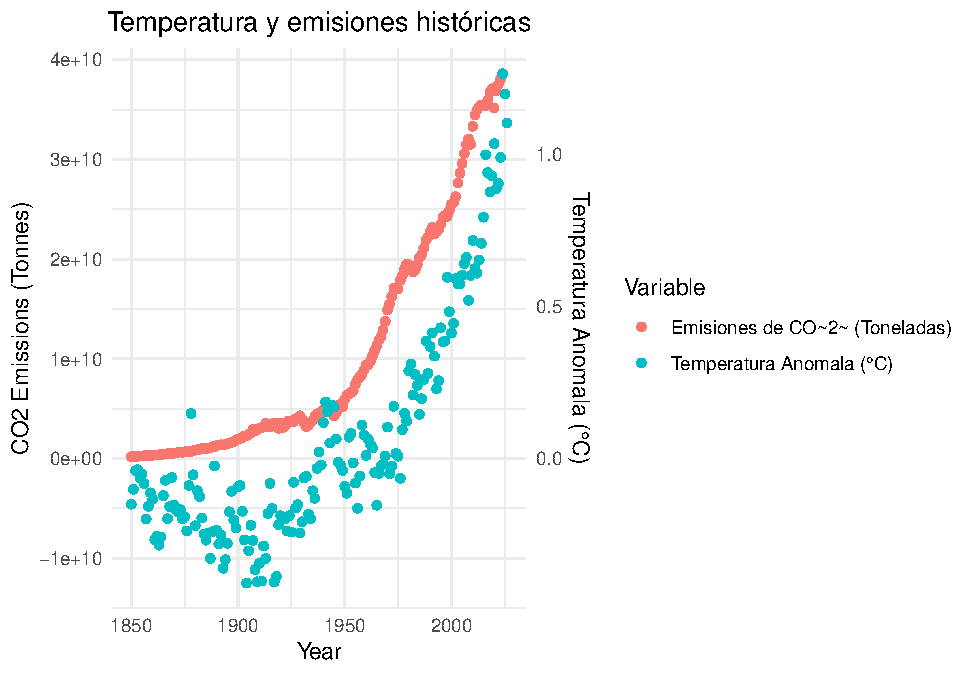
\includegraphics[keepaspectratio]{proyecto-Fabian_files/figure-latex/1-1.pdf}}
\caption{\label{fig:1}Comportamiento anual de la Emisión total de CO\textsubscript{2} y Temperatura Anómala}
\end{figure}

\begin{Shaded}
\begin{Highlighting}[]
\FunctionTok{ggplot}\NormalTok{(yearly\_data, }\FunctionTok{aes}\NormalTok{(}\AttributeTok{x =}\NormalTok{ CO2\_emissions, }\AttributeTok{y =}\NormalTok{ mean\_temperature\_anomaly)) }\SpecialCharTok{+}
  \FunctionTok{geom\_point}\NormalTok{() }\SpecialCharTok{+}
  \FunctionTok{geom\_smooth}\NormalTok{(}\AttributeTok{method =} \StringTok{"lm"}\NormalTok{, }\AttributeTok{se =} \ConstantTok{FALSE}\NormalTok{) }\SpecialCharTok{+}
  \FunctionTok{labs}\NormalTok{(}
    \AttributeTok{x =} \StringTok{"Emisiones de CO2 (Toneladas)"}\NormalTok{,}
    \AttributeTok{y =} \StringTok{"Temperatura Anomala"}\NormalTok{,}
    \AttributeTok{title =} \StringTok{"CO2 vs Temperatura Anomala"}
\NormalTok{  ) }\SpecialCharTok{+}
  \FunctionTok{theme\_minimal}\NormalTok{()}\SpecialCharTok{+}
  \FunctionTok{theme}\NormalTok{(}\AttributeTok{plot.title =} \FunctionTok{element\_text}\NormalTok{(}\AttributeTok{hjust =} \FloatTok{0.5}\NormalTok{))}
\end{Highlighting}
\end{Shaded}

\begin{figure}
\centering
\pandocbounded{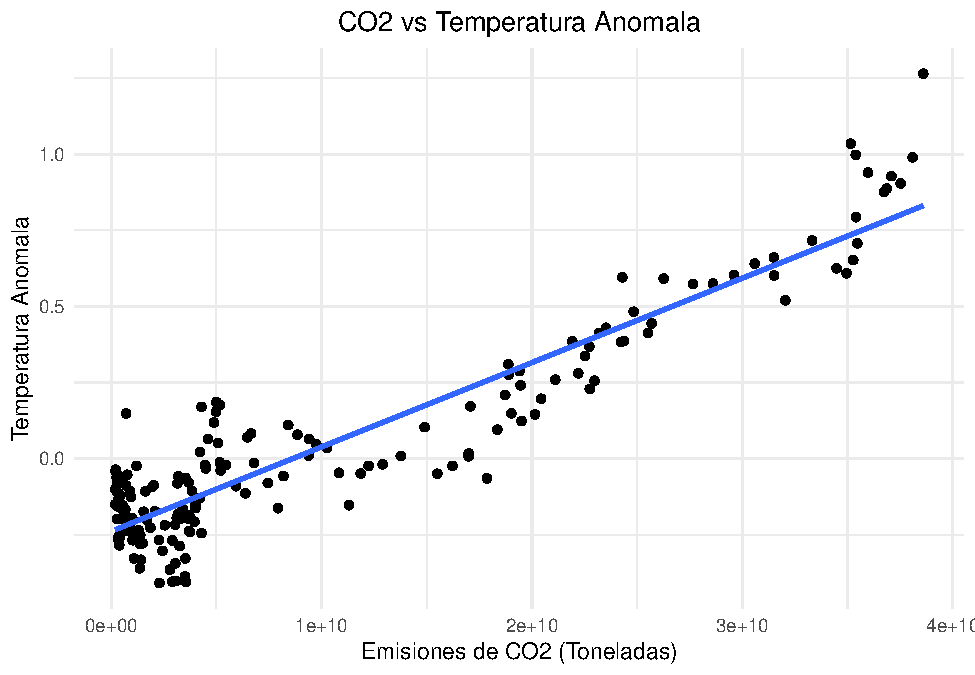
\includegraphics[keepaspectratio]{proyecto-Fabian_files/figure-latex/2-1.pdf}}
\caption{\label{fig:2}Gráfico de Dispersión de la Emisión Total de CO\textsubscript{2} vs Temperatura Anómala}
\end{figure}

\section{\texorpdfstring{Emisiones de CO\textsubscript{2} y el desarrollo ecónomico.}{Emisiones de CO2 y el desarrollo ecónomico.}}\label{emisiones-de-co2-y-el-desarrollo-ecuxf3nomico.}

Tras establecer la relación entre las emisiones y el incremento en la temperatura anomala, nuestro análisis continua con la busqueda de una relación entre el desempeño económico de un país y los niveles de emisiones de CO2 que este genera. El análisis histórico revela diferencias estructurales entre grupos de ingreso \ref{fig:4}:

\begin{itemize}
\tightlist
\item
  Los países de altos ingresos presentan un crecimiento temprano y acelerado de emisiones per cápita desde el siglo XIX, alcanzando niveles elevados durante el siglo XX, seguido de una leve estabilización o reducción reciente.
\item
  Los países de ingresos medios, especialmente medios-altos, muestran un crecimiento tardío pero pronunciado a partir de mediados del siglo XX, coincidiendo con procesos de industrialización acelerada.
\item
  Los países de bajos ingresos mantienen niveles bajos de emisiones per cápita, con incrementos modestos en algunos casos.
\end{itemize}

\begin{Shaded}
\begin{Highlighting}[]
\FunctionTok{ggplot}\NormalTok{(income\_data, }\FunctionTok{aes}\NormalTok{(}\AttributeTok{x =}\NormalTok{ Year, }\AttributeTok{y =} \StringTok{\textasciigrave{}}\AttributeTok{CO2 per capita}\StringTok{\textasciigrave{}}\NormalTok{, }\AttributeTok{color =}\NormalTok{ Entity)) }\SpecialCharTok{+}
  \FunctionTok{geom\_line}\NormalTok{(}\AttributeTok{size =} \DecValTok{1}\NormalTok{) }\SpecialCharTok{+}
  \FunctionTok{labs}\NormalTok{(}
    \AttributeTok{title =} \StringTok{"CO2 Emissions per Capita Over Time"}\NormalTok{,}
    \AttributeTok{x =} \StringTok{"Year"}\NormalTok{,}
    \AttributeTok{y =} \StringTok{"CO2 Emissions"}\NormalTok{,}
    \AttributeTok{color =} \StringTok{"Income Group"}
\NormalTok{  ) }\SpecialCharTok{+}
  \FunctionTok{theme\_minimal}\NormalTok{()}\SpecialCharTok{+}
  \FunctionTok{theme}\NormalTok{(}\AttributeTok{plot.title =} \FunctionTok{element\_text}\NormalTok{(}\AttributeTok{hjust =} \FloatTok{0.5}\NormalTok{))}
\end{Highlighting}
\end{Shaded}

\begin{figure}
\centering
\pandocbounded{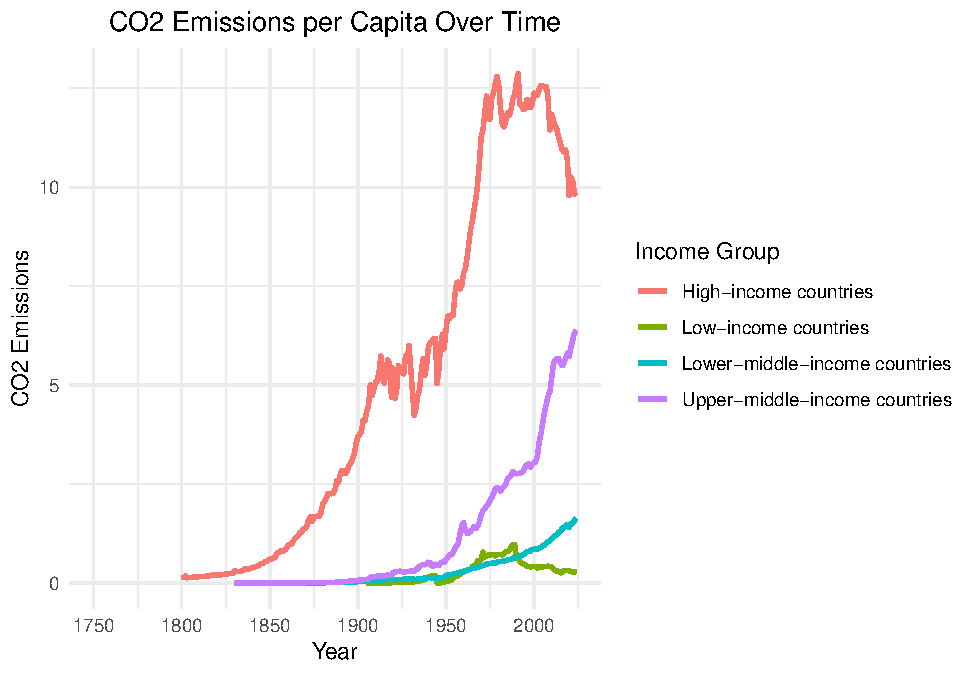
\includegraphics[keepaspectratio]{proyecto-Fabian_files/figure-latex/4-1.pdf}}
\caption{\label{fig:4}Emisiones per Capita categorizadas por Grupo Económico}
\end{figure}

El comportamiento de las emisiones totales \ref{fig:3} refuerza los hallazgos anteriores. Los países de ingresos altos dominan las emisiones históricas, con reducciones en los últimos años producto de implementación de medidas de reducción de emisiones. Caso contrario, los países de ingresos medios-altos muestran un crecimiento acelerado, llegando a superar o acercarse a los niveles de los países desarrollados, mostrando que la implementación de medidas de reducción de emisiones no ha sido prioritario en este etipo de países, probablemente ocasionada por la reticencia a impactar su crecimiento económico y verse relegados frente a otros países. Los países de bajos ingresos, finalmente, contribuyen marginalmente al total global.

Se puede establecer, entonces, que la cronología de las emisiones refleja claramente las etapas de industrialización. La industrialización temprana en países desarrollados causaron que históricamente fueran los principales actores en la producción de emisiones, pero que en los últimos tiempos, la industrialización tardía en economías emergentes ha causado un crecimiento en su papel global de generación de emisiones.

\begin{Shaded}
\begin{Highlighting}[]
\FunctionTok{ggplot}\NormalTok{(income\_data, }\FunctionTok{aes}\NormalTok{(}\AttributeTok{x =}\NormalTok{ Year, }\AttributeTok{y =} \StringTok{\textasciigrave{}}\AttributeTok{CO2 emissions}\StringTok{\textasciigrave{}}\NormalTok{, }\AttributeTok{color =}\NormalTok{ Entity)) }\SpecialCharTok{+}
  \FunctionTok{geom\_line}\NormalTok{(}\AttributeTok{size =} \DecValTok{1}\NormalTok{) }\SpecialCharTok{+}
  \FunctionTok{labs}\NormalTok{(}
    \AttributeTok{title =} \StringTok{"CO2 Emissions Total Over Time"}\NormalTok{,}
    \AttributeTok{x =} \StringTok{"Year"}\NormalTok{,}
    \AttributeTok{y =} \StringTok{"CO2 Emissions"}\NormalTok{,}
    \AttributeTok{color =} \StringTok{"Income Group"}
\NormalTok{  ) }\SpecialCharTok{+}
  \FunctionTok{theme\_minimal}\NormalTok{()}\SpecialCharTok{+}
  \FunctionTok{theme}\NormalTok{(}\AttributeTok{plot.title =} \FunctionTok{element\_text}\NormalTok{(}\AttributeTok{hjust =} \FloatTok{0.5}\NormalTok{))}
\end{Highlighting}
\end{Shaded}

\begin{figure}
\centering
\pandocbounded{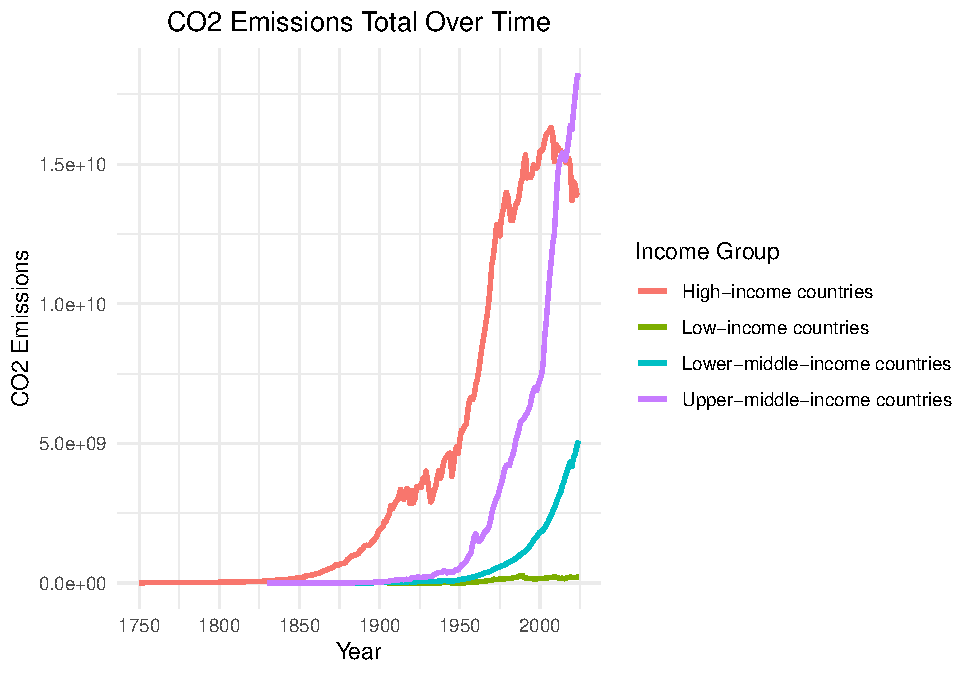
\includegraphics[keepaspectratio]{proyecto-Fabian_files/figure-latex/3-1.pdf}}
\caption{\label{fig:3}Gráfico de Dispersión de la Emisión Total de CO\textsubscript{2} vs Temperatura Anómala}
\end{figure}

Para complementar este análisis, usamos un diagrama de dispersión entre PIB y emisiones de CO₂, tanto total \ref{fig:5} como per capita \ref{fig:6}. Estos diagramas evidencian una relación positiva, aunque con alta dispersión. Las economías de gran escala concentran la mayor parte de las emisiones globales.

Sin embargo, la variabilidad observada indica que no todos los países emiten al mismo nivel. Observamos Existen economías con PIB medio cuyas emisiones superan a las de países con alto PIB, lo que sugiere diferencias en eficiencia energética, matriz energética o políticas ambientales. Pero el panorama global es clara, y la tendencia año a año muestra que los países con mayor poder ecónomico son los principales responsables de la generación de emisiones a nivel global.

\begin{Shaded}
\begin{Highlighting}[]
\FunctionTok{ggplot}\NormalTok{(gdp\_joined\_data }\SpecialCharTok{\%\textgreater{}\%} \FunctionTok{filter}\NormalTok{(Year }\SpecialCharTok{\%in\%} \FunctionTok{c}\NormalTok{(}\DecValTok{1990}\NormalTok{, }\DecValTok{2000}\NormalTok{, }\DecValTok{2010}\NormalTok{)), }\FunctionTok{aes}\NormalTok{(}\AttributeTok{x =}\NormalTok{ GDP, }\AttributeTok{y =} \StringTok{\textasciigrave{}}\AttributeTok{Annual CO2 emissions}\StringTok{\textasciigrave{}}\NormalTok{)) }\SpecialCharTok{+}
  \FunctionTok{geom\_point}\NormalTok{() }\SpecialCharTok{+}
  \FunctionTok{geom\_smooth}\NormalTok{(}\AttributeTok{method =} \StringTok{"lm"}\NormalTok{, }\AttributeTok{se =} \ConstantTok{FALSE}\NormalTok{) }\SpecialCharTok{+}
  \FunctionTok{facet\_grid}\NormalTok{(. }\SpecialCharTok{\textasciitilde{}}\NormalTok{ Year) }\SpecialCharTok{+}
  \FunctionTok{labs}\NormalTok{(}
    \AttributeTok{x =} \StringTok{"GDP (USD)"}\NormalTok{,}
    \AttributeTok{y =} \StringTok{"CO2 Emissions"}\NormalTok{,}
    \AttributeTok{title =} \StringTok{"GDP vs CO2 a lo largo de los años"}
\NormalTok{  ) }\SpecialCharTok{+}
  \FunctionTok{theme\_minimal}\NormalTok{()}\SpecialCharTok{+}
  \FunctionTok{theme}\NormalTok{(}\AttributeTok{plot.title =} \FunctionTok{element\_text}\NormalTok{(}\AttributeTok{hjust =} \FloatTok{0.5}\NormalTok{))}
\end{Highlighting}
\end{Shaded}

\begin{figure}
\centering
\pandocbounded{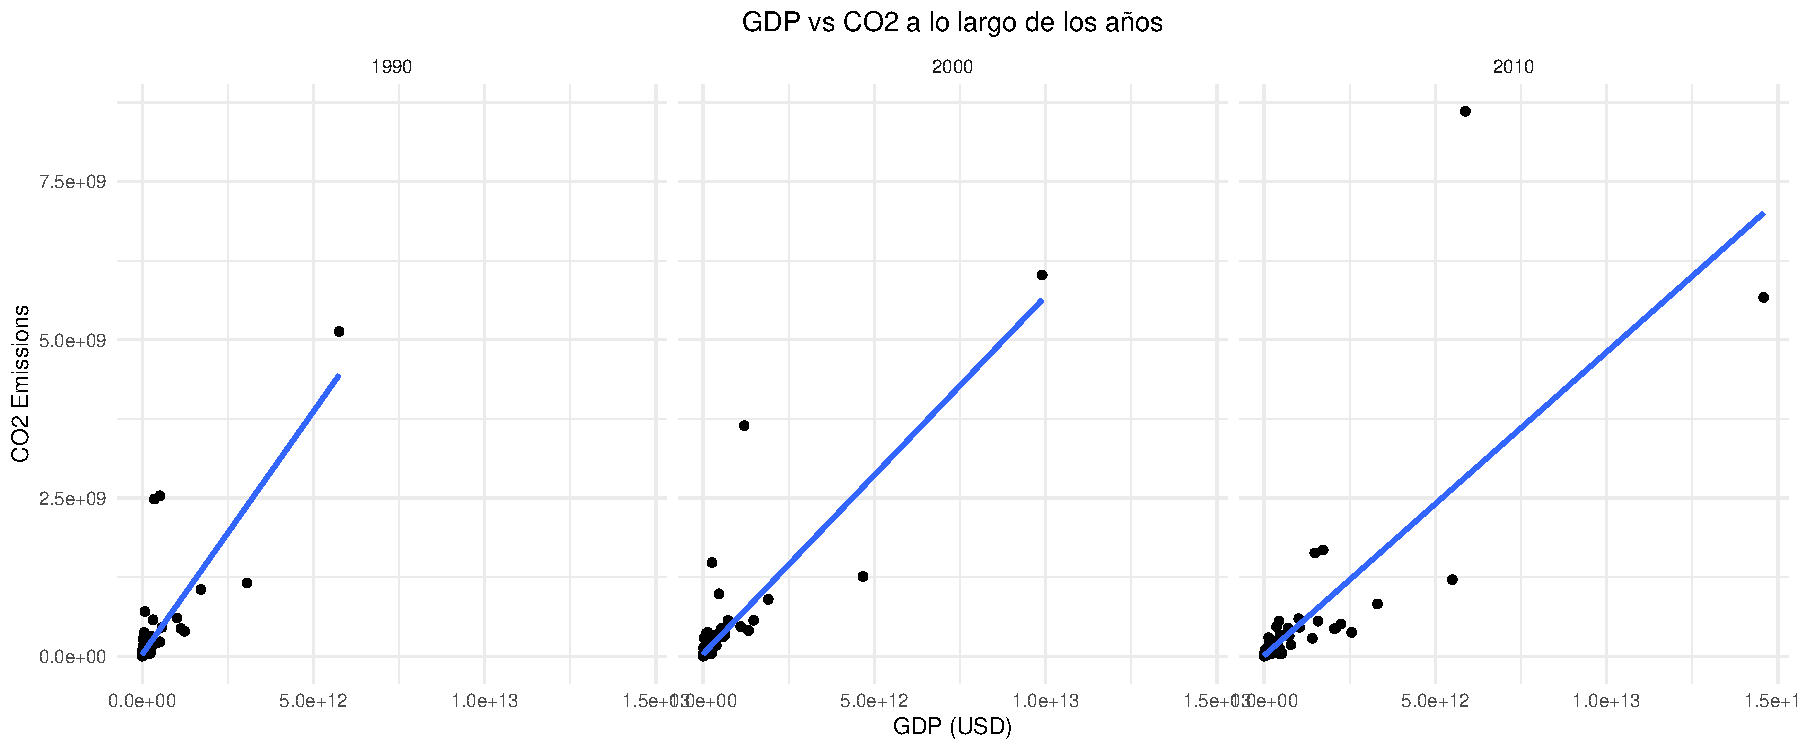
\includegraphics[keepaspectratio]{proyecto-Fabian_files/figure-latex/5-1.pdf}}
\caption{\label{fig:5}Correlación GDP vs Emisiones de CO\textsubscript{2}}
\end{figure}

\begin{Shaded}
\begin{Highlighting}[]
\NormalTok{gdp\_joined\_data}\SpecialCharTok{$}\NormalTok{co2\_per\_capita }\OtherTok{=}\NormalTok{ gdp\_joined\_data}\SpecialCharTok{$}\StringTok{\textasciigrave{}}\AttributeTok{Annual CO2 emissions}\StringTok{\textasciigrave{}}\SpecialCharTok{/}\NormalTok{gdp\_joined\_data}\SpecialCharTok{$}\NormalTok{Population}

\FunctionTok{ggplot}\NormalTok{(gdp\_joined\_data }\SpecialCharTok{\%\textgreater{}\%} \FunctionTok{filter}\NormalTok{(Year }\SpecialCharTok{\%in\%} \FunctionTok{c}\NormalTok{(}\DecValTok{1990}\NormalTok{, }\DecValTok{2000}\NormalTok{, }\DecValTok{2010}\NormalTok{)), }\FunctionTok{aes}\NormalTok{(}\AttributeTok{x =} \StringTok{\textasciigrave{}}\AttributeTok{GDP per Capita}\StringTok{\textasciigrave{}}\NormalTok{, }\AttributeTok{y =}\NormalTok{ co2\_per\_capita)) }\SpecialCharTok{+}
  \FunctionTok{geom\_point}\NormalTok{() }\SpecialCharTok{+}
  \FunctionTok{geom\_smooth}\NormalTok{(}\AttributeTok{method =} \StringTok{"lm"}\NormalTok{, }\AttributeTok{se =} \ConstantTok{FALSE}\NormalTok{) }\SpecialCharTok{+}
  \FunctionTok{facet\_grid}\NormalTok{(. }\SpecialCharTok{\textasciitilde{}}\NormalTok{ Year) }\SpecialCharTok{+}
  \FunctionTok{labs}\NormalTok{(}
    \AttributeTok{x =} \StringTok{"GDP per Capita (USD per Person)"}\NormalTok{,}
    \AttributeTok{y =} \StringTok{"CO2 Emissions per capita"}\NormalTok{,}
    \AttributeTok{title =} \StringTok{"GDP per Capita vs CO2 per capita"}
\NormalTok{  ) }\SpecialCharTok{+}
  \FunctionTok{theme\_minimal}\NormalTok{()}\SpecialCharTok{+}
  \FunctionTok{theme}\NormalTok{(}\AttributeTok{plot.title =} \FunctionTok{element\_text}\NormalTok{(}\AttributeTok{hjust =} \FloatTok{0.5}\NormalTok{))}
\end{Highlighting}
\end{Shaded}

\begin{figure}
\centering
\pandocbounded{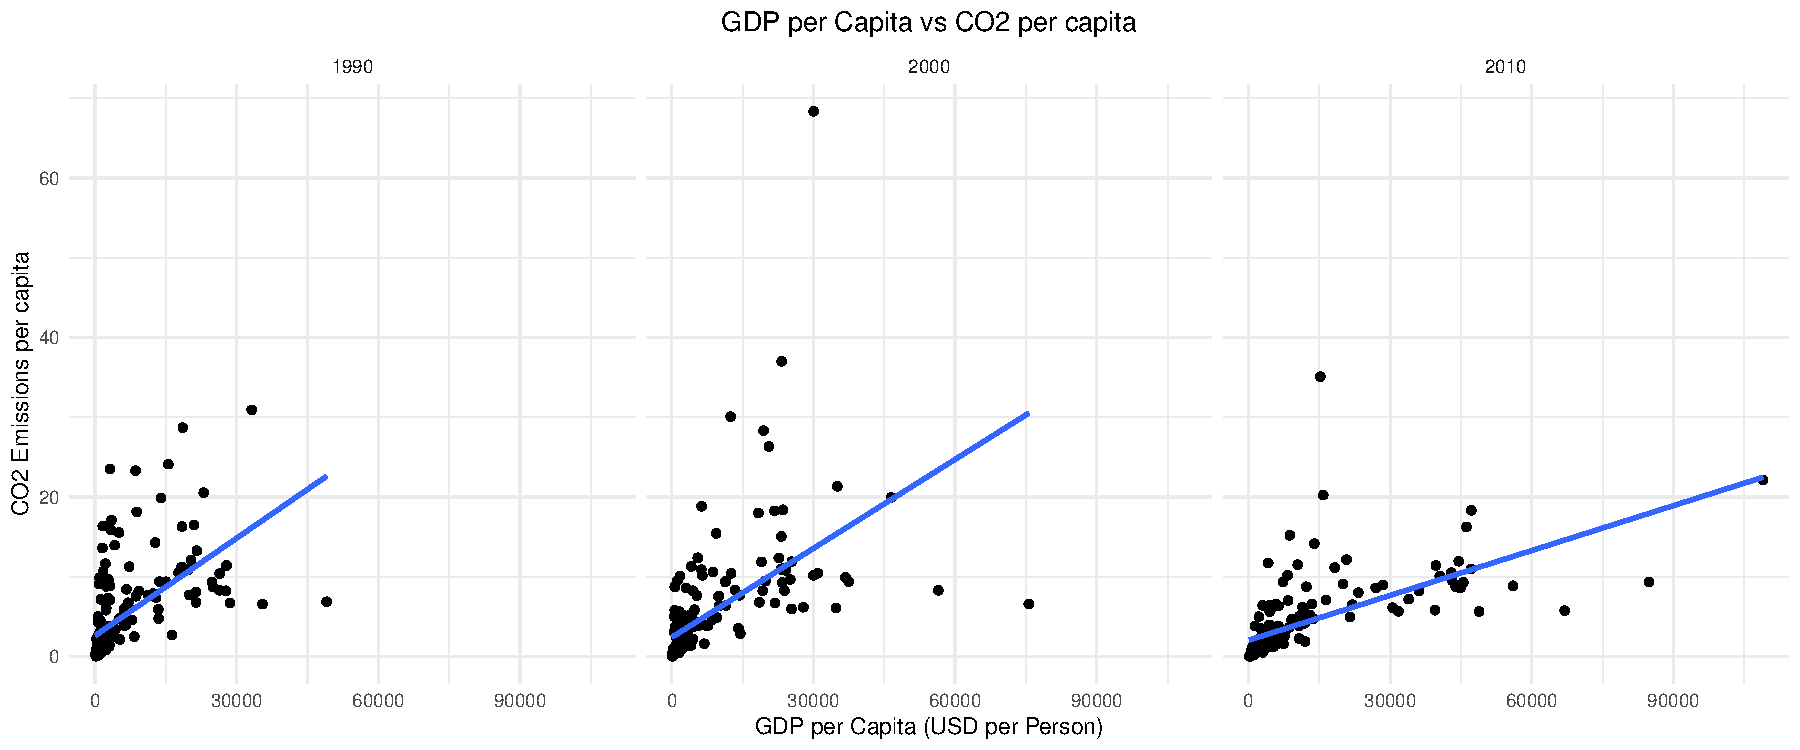
\includegraphics[keepaspectratio]{proyecto-Fabian_files/figure-latex/6-1.pdf}}
\caption{\label{fig:6}Correlación GDP per Capita vs Emisiones de CO\textsubscript{2} per Capita}
\end{figure}

\section{Analisis Regional}\label{analisis-regional}

\begin{Shaded}
\begin{Highlighting}[]
\NormalTok{gdp\_joined\_data }\SpecialCharTok{\%\textgreater{}\%} 
  \FunctionTok{inner\_join}\NormalTok{(country\_data, }\AttributeTok{by=}\StringTok{"Country code"}\NormalTok{) }\SpecialCharTok{\%\textgreater{}\%} 
  \FunctionTok{select}\NormalTok{(}\SpecialCharTok{{-}}\StringTok{\textasciigrave{}}\AttributeTok{Country name}\StringTok{\textasciigrave{}}\NormalTok{) }\OtherTok{{-}\textgreater{}}\NormalTok{ gdp\_joined\_data2}
  
\NormalTok{gdp\_joined\_data2 }\SpecialCharTok{\%\textgreater{}\%} 
  \FunctionTok{group\_by}\NormalTok{(Region, Year) }\SpecialCharTok{\%\textgreater{}\%} 
  \FunctionTok{summarize}\NormalTok{(}\AttributeTok{total\_emission =} \FunctionTok{sum}\NormalTok{(}\StringTok{\textasciigrave{}}\AttributeTok{Annual CO2 emissions}\StringTok{\textasciigrave{}}\NormalTok{), }\AttributeTok{total\_gdp =} \FunctionTok{sum}\NormalTok{(GDP))}\OtherTok{{-}\textgreater{}}\NormalTok{ gdp\_joined\_data\_region}
\end{Highlighting}
\end{Shaded}

Trasladamos nuestro análisis a nivel regional, donde podemos evidenciar 3 principales actores en la producción de emisiones (\ref{fig:7}) y desarrollo económico (\ref{fig:8}) a nivel global:

\begin{itemize}
\tightlist
\item
  Pacifico y Asia Oriental
\item
  Europa y Asia Central
\item
  América del Norte
\end{itemize}

La tendencia más notable corresponde a Asia Oriental y el Pacífico, cuyas emisiones crecen de forma exponencial ---de aproximadamente 4.5 × 10⁹ a 1.2 × 10¹⁰ toneladas--- mientras su PIB se expande significativamente, aunque sin alcanzar los niveles absolutos de Europa o América del Norte hacia 2010. Esta asimetría revela una estructura productiva con alta producción de carbono, propia de economías en fase de industrialización acelerada. Europa y Asia Central, en contraste, muestra una reducción de emisiones durante los años noventa seguida de estabilización, mientras mantiene el mayor PIB regional del período. América del Norte exhibe emisiones crecientes de forma estable con leve decrecimiento hacia 2010. Las regiones de menor desarrollo ---América Latina, Asia del Sur, Oriente Medio y África Subsahariana--- registran emisiones absolutas bajas pero con tendencias ascendentes moderadas, anticipando que su industrialización futura será un factor determinante en las trayectorias globales de carbono.

El análisis conjunto permite establecer tres conclusiones centrales. Primero, existe una correlación positiva entre industrialización acelerada e incremento de emisiones, siendo Asia Oriental la evidencia más contundente del período. Segundo, las economías post-industriales exhiben un desacoplamiento progresivo entre PIB y emisiones, pero manteniendo una participación considerable en el total global. Tercero, la intensidad de carbono ---emisiones por unidad de PIB--- resulta más informativa que las emisiones absolutas para evaluar la eficiencia ambiental de una economía, ya que niveles bajos de emisión pueden reflejar simplemente un bajo nivel de desarrollo y no una transición hacia modelos productivos más limpios.

\begin{Shaded}
\begin{Highlighting}[]
\FunctionTok{ggplot}\NormalTok{(gdp\_joined\_data\_region, }\FunctionTok{aes}\NormalTok{(}\AttributeTok{x =}\NormalTok{ Year, }\AttributeTok{y =}\NormalTok{ total\_emission, }\AttributeTok{color =}\NormalTok{ Region)) }\SpecialCharTok{+}
  \FunctionTok{geom\_line}\NormalTok{(}\AttributeTok{size =} \DecValTok{1}\NormalTok{) }\SpecialCharTok{+}
  \FunctionTok{labs}\NormalTok{(}
    \AttributeTok{title =} \StringTok{"Histórico de Emisiones de CO2 por Región"}\NormalTok{,}
    \AttributeTok{x =} \StringTok{"Año"}\NormalTok{,}
    \AttributeTok{y =} \StringTok{"Emisiones de CO2 (toneladas)"}\NormalTok{,}
    \AttributeTok{color =} \StringTok{"Región"}
\NormalTok{  ) }\SpecialCharTok{+}
  \FunctionTok{theme\_minimal}\NormalTok{()}\SpecialCharTok{+}
  \FunctionTok{theme}\NormalTok{(}\AttributeTok{plot.title =} \FunctionTok{element\_text}\NormalTok{(}\AttributeTok{hjust =} \FloatTok{0.5}\NormalTok{))}
\end{Highlighting}
\end{Shaded}

\begin{figure}
\centering
\pandocbounded{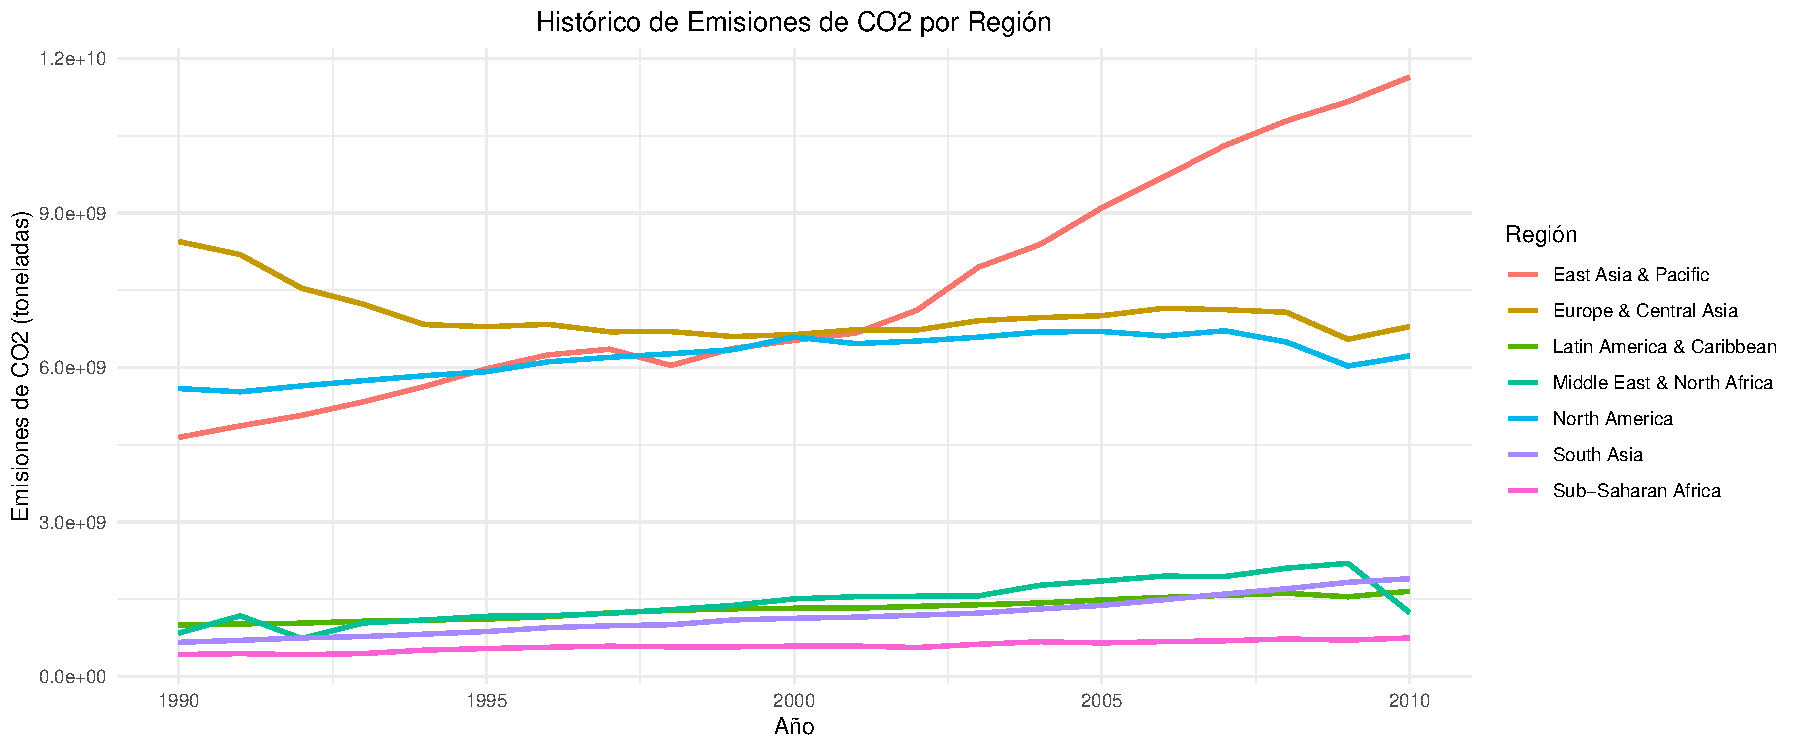
\includegraphics[keepaspectratio]{proyecto-Fabian_files/figure-latex/7-1.pdf}}
\caption{\label{fig:7}Emisiones por Región}
\end{figure}

\begin{Shaded}
\begin{Highlighting}[]
\FunctionTok{ggplot}\NormalTok{(gdp\_joined\_data\_region, }\FunctionTok{aes}\NormalTok{(}\AttributeTok{x =}\NormalTok{ Year, }\AttributeTok{y =}\NormalTok{ total\_gdp, }\AttributeTok{color =}\NormalTok{ Region)) }\SpecialCharTok{+}
  \FunctionTok{geom\_line}\NormalTok{(}\AttributeTok{size =} \DecValTok{1}\NormalTok{) }\SpecialCharTok{+}
  \FunctionTok{labs}\NormalTok{(}
    \AttributeTok{title =} \StringTok{"Histórico de PIB por Región"}\NormalTok{,}
    \AttributeTok{x =} \StringTok{"Año"}\NormalTok{,}
    \AttributeTok{y =} \StringTok{"PIB (USD)"}\NormalTok{,}
    \AttributeTok{color =} \StringTok{"Región"}
\NormalTok{  ) }\SpecialCharTok{+}
  \FunctionTok{theme\_minimal}\NormalTok{()}\SpecialCharTok{+}
  \FunctionTok{theme}\NormalTok{(}\AttributeTok{plot.title =} \FunctionTok{element\_text}\NormalTok{(}\AttributeTok{hjust =} \FloatTok{0.5}\NormalTok{))}
\end{Highlighting}
\end{Shaded}

\pandocbounded{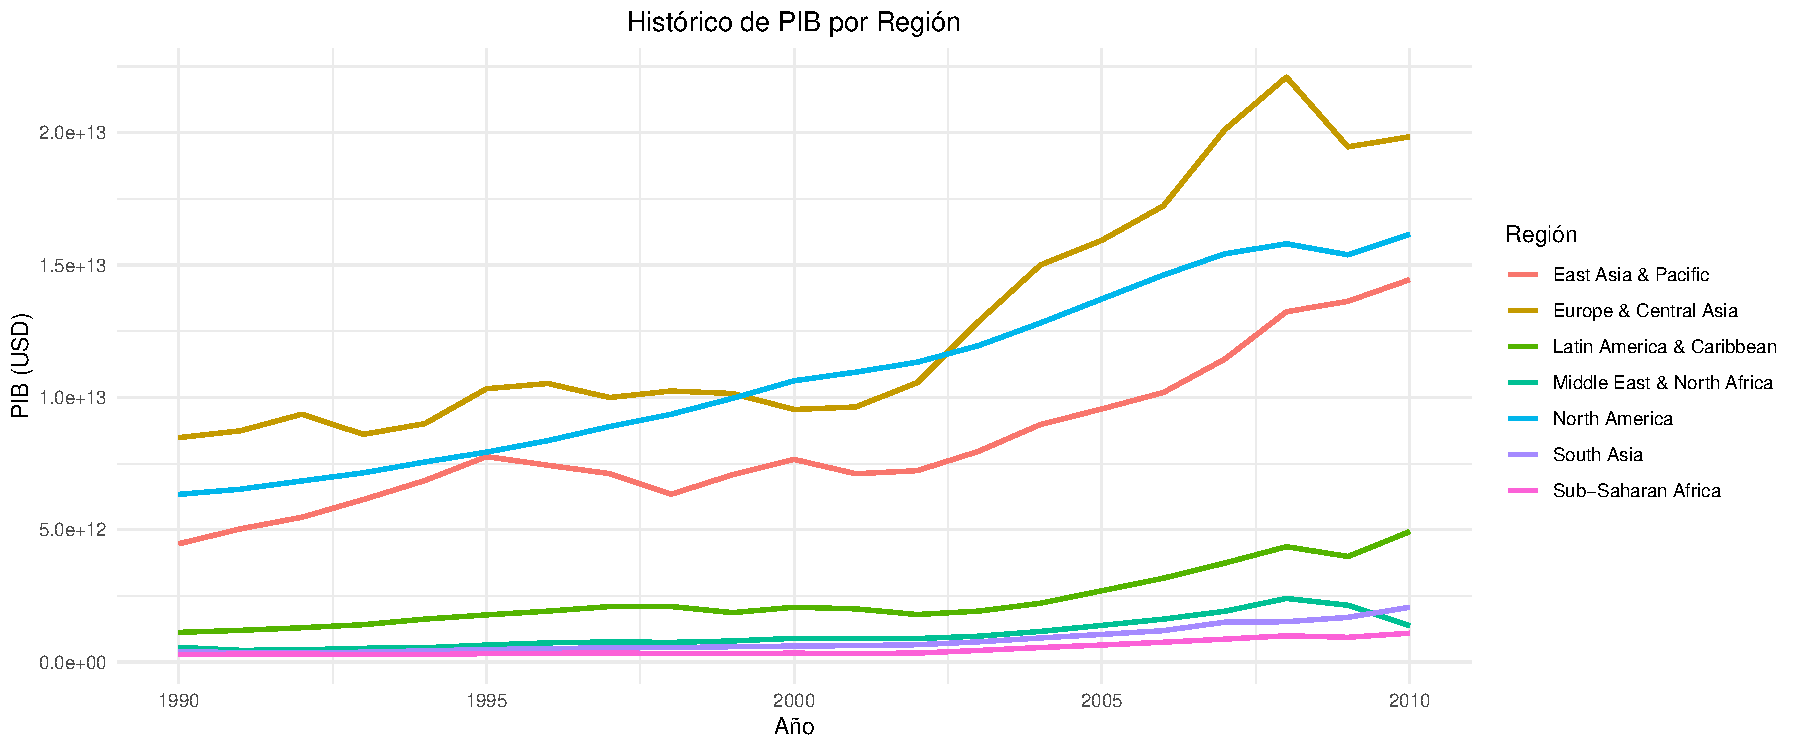
\includegraphics[keepaspectratio]{proyecto-Fabian_files/figure-latex/8-1.pdf}}
Finalmente, analizamos la composición por niveles de ingreso de los países en cada región (\ref{fig:9}), ordenadas de mayor a menor participación de economías de alto ingreso. Observamos que las regiones con mayor proporción de países de alto ingreso (OCDE) son las 3 regiones que encontramos contruyen mayoritariamente a la emisión de CO\textsubscript{2}. La información provista por esta gráfica se alinea con lo visto en (\ref{fig:7}) y (\ref{fig:8}).

\begin{Shaded}
\begin{Highlighting}[]
\NormalTok{country\_data }\SpecialCharTok{\%\textgreater{}\%} 
  \FunctionTok{filter}\NormalTok{(Region }\SpecialCharTok{!=} \StringTok{"Aggregates"}\NormalTok{) }\SpecialCharTok{\%\textgreater{}\%} 
  \FunctionTok{count}\NormalTok{(Region, }\StringTok{\textasciigrave{}}\AttributeTok{Income group}\StringTok{\textasciigrave{}}\NormalTok{, }\AttributeTok{name =} \StringTok{"n\_count"}\NormalTok{) }\OtherTok{{-}\textgreater{}}\NormalTok{ income\_group\_per\_region}

\NormalTok{region\_order }\OtherTok{\textless{}{-}}\NormalTok{ country\_data }\SpecialCharTok{\%\textgreater{}\%}
  \FunctionTok{group\_by}\NormalTok{(Region) }\SpecialCharTok{\%\textgreater{}\%}
  \FunctionTok{summarise}\NormalTok{(}
    \AttributeTok{total =} \FunctionTok{n}\NormalTok{(),}
    \AttributeTok{high\_income =} \FunctionTok{sum}\NormalTok{(}\StringTok{\textasciigrave{}}\AttributeTok{Income group}\StringTok{\textasciigrave{}} \SpecialCharTok{==} \StringTok{"High income: OECD"}\NormalTok{, }\AttributeTok{na.rm =} \ConstantTok{TRUE}\NormalTok{),}
    \AttributeTok{prop\_high =}\NormalTok{ high\_income }\SpecialCharTok{/}\NormalTok{ total,}
    \AttributeTok{.groups =} \StringTok{"drop"}
\NormalTok{  )}

\NormalTok{plot\_data }\OtherTok{\textless{}{-}}\NormalTok{ income\_group\_per\_region }\SpecialCharTok{\%\textgreater{}\%}
  \FunctionTok{left\_join}\NormalTok{(region\_order, }\AttributeTok{by =} \StringTok{"Region"}\NormalTok{) }\SpecialCharTok{\%\textgreater{}\%}
  \FunctionTok{mutate}\NormalTok{(}\AttributeTok{Region =} \FunctionTok{reorder}\NormalTok{(Region, prop\_high))}

\FunctionTok{ggplot}\NormalTok{(plot\_data, }
       \FunctionTok{aes}\NormalTok{(}\AttributeTok{x =}\NormalTok{ Region, }\AttributeTok{y =}\NormalTok{ n\_count, }\AttributeTok{fill =} \StringTok{\textasciigrave{}}\AttributeTok{Income group}\StringTok{\textasciigrave{}}\NormalTok{)) }\SpecialCharTok{+}
  \FunctionTok{geom\_bar}\NormalTok{(}\AttributeTok{stat =} \StringTok{"identity"}\NormalTok{) }\SpecialCharTok{+}
  \FunctionTok{coord\_flip}\NormalTok{() }\SpecialCharTok{+}
  \FunctionTok{labs}\NormalTok{(}
    \AttributeTok{x =} \StringTok{"Región"}\NormalTok{,}
    \AttributeTok{y =} \StringTok{"Número de Países"}\NormalTok{,}
    \AttributeTok{title =} \StringTok{"Grupo de Ingresos por región"}
\NormalTok{  ) }\SpecialCharTok{+}
  \FunctionTok{theme\_minimal}\NormalTok{()}\SpecialCharTok{+}
  \FunctionTok{theme}\NormalTok{(}\AttributeTok{plot.title =} \FunctionTok{element\_text}\NormalTok{(}\AttributeTok{hjust =} \FloatTok{0.5}\NormalTok{))}
\end{Highlighting}
\end{Shaded}

\begin{figure}
\centering
\pandocbounded{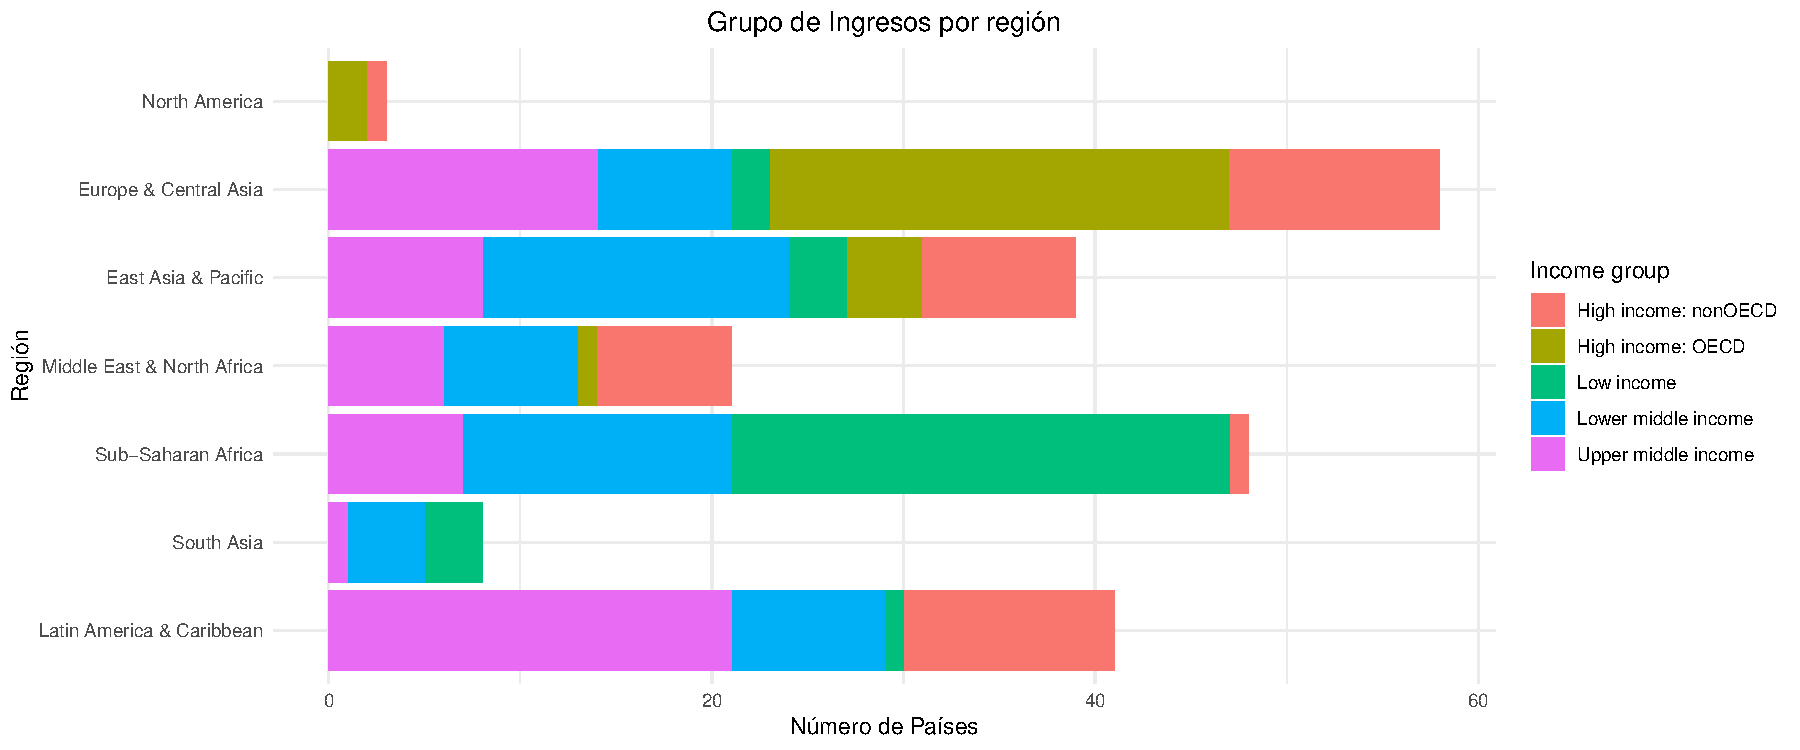
\includegraphics[keepaspectratio]{proyecto-Fabian_files/figure-latex/9-1.pdf}}
\caption{\label{fig:9}Distribución económica por región}
\end{figure}

\section{Analisis de distribución de emisiones regional y económica}\label{analisis-de-distribuciuxf3n-de-emisiones-regional-y-econuxf3mica}

Generamos 2 diagramas de caja (boxplots) \ref{fig:7} y \ref{fig:8} con el objetivo de profundizar en la heterogeneidad interna de las emisiones de CO₂, desagregando la información por grupo de ingreso y por región respectivamente. Para facilidad de nuestro análisis y evitar incorporar ruido por cambios temporales, filtramos la información para el año 2010.

Por grupo de ingreso, el resultado más destacado es la elevada dispersión interna del grupo de alto ingreso OCDE, cuya caja intercuartílica se extiende notablemente por encima de los demás grupos, con un valor atípico (outlier) que supera los 5 × 10⁹ toneladas ---atribuible presumiblemente a Estados Unidos o un emisor de escala comparable. Los grupos de ingreso bajo e ingreso medio-bajo presentan cajas prácticamente colapsadas sobre el eje horizontal, con medianas cercanas a cero y outliers aislados que representan países de gran población como India o Nigeria. El grupo de ingreso medio-alto muestra un outlier superior cercano a los 8 × 10⁹ toneladas, el más alto del gráfico, consistente con la posición de China en ese grupo de clasificación para 2010. Este hallazgo indica algo: las mayores emisiones absolutas en 2010 no provienen de los países de mayor ingreso per cápita, sino de economías en transición de ingreso medio-alto con grandes bases industriales y poblacionales.

Por región, el contraste es aún más pronunciado. América del Norte exhibe la distribución más amplia con diferencia: su caja intercuartílica abarca el rango entre aproximadamente 2 × 10⁹ y 5 × 10⁹ toneladas, con una mediana en torno a 3 × 10⁹, lo que refleja que incluso el país mediano de esa región ---compuesta por muy pocos países de alta emisión individual--- genera volúmenes extraordinariamente elevados. Asia Oriental y el Pacífico presenta una caja comprimida pero con un outlier superior cercano a los 8 × 10⁹ toneladas, el valor más alto del gráfico, coherente con la presencia de China como emisor dominante dentro de una región por lo demás heterogénea. Todas las demás regiones ---Europa y Asia Central, América Latina, Oriente Medio, Asia del Sur y África Subsahariana--- muestran distribuciones extremadamente comprimidas con medianas próximas a cero, indicando que la gran mayoría de sus países son emisores menores en términos absolutos, aunque con outliers aislados de relevancia.

La lectura conjunta de ambos gráficos refuerza una conclusión: la distribución de emisiones de CO\textsubscript{4} es profundamente asimétrica tanto entre regiones como dentro de los grupos de ingreso, con un número reducido de países ---caracterizados por grandes economías industriales, alta población o abundancia de recursos fósiles--- concentrando la mayor parte de las emisiones globales. Esta concentración implica que las políticas de mitigación climática tienen un potencial de impacto desproporcionadamente mayor si se focalizan en dichos emisores dominantes, independientemente de su clasificación regional o de ingreso.

\begin{Shaded}
\begin{Highlighting}[]
\FunctionTok{ggplot}\NormalTok{(gdp\_joined\_data2[gdp\_joined\_data2}\SpecialCharTok{$}\NormalTok{Year }\SpecialCharTok{==} \DecValTok{2010}\NormalTok{,], }\FunctionTok{aes}\NormalTok{(}\AttributeTok{x =} \FunctionTok{factor}\NormalTok{(Region), }\AttributeTok{y =} \StringTok{\textasciigrave{}}\AttributeTok{Annual CO2 emissions}\StringTok{\textasciigrave{}}\NormalTok{, }\AttributeTok{fill =}\NormalTok{ Region)) }\SpecialCharTok{+}
  \FunctionTok{geom\_boxplot}\NormalTok{() }\SpecialCharTok{+}
  \FunctionTok{labs}\NormalTok{(}
    \AttributeTok{x =} \StringTok{"Región"}\NormalTok{,}
    \AttributeTok{y =} \StringTok{"Emisiones de CO2"}\NormalTok{,}
    \AttributeTok{title =} \StringTok{"Distribución de las emisiones de CO2 por región en 2010"}
\NormalTok{  ) }\SpecialCharTok{+}
  \FunctionTok{theme\_minimal}\NormalTok{() }\SpecialCharTok{+}
  \FunctionTok{theme}\NormalTok{(}
    \AttributeTok{axis.text.x =} \FunctionTok{element\_blank}\NormalTok{(),}
    \AttributeTok{axis.ticks.x =} \FunctionTok{element\_blank}\NormalTok{(),}
    \AttributeTok{plot.title =} \FunctionTok{element\_text}\NormalTok{(}\AttributeTok{hjust =} \FloatTok{0.5}\NormalTok{)}
\NormalTok{  )}\SpecialCharTok{+}
  \FunctionTok{theme}\NormalTok{()}
\end{Highlighting}
\end{Shaded}

\begin{figure}
\centering
\pandocbounded{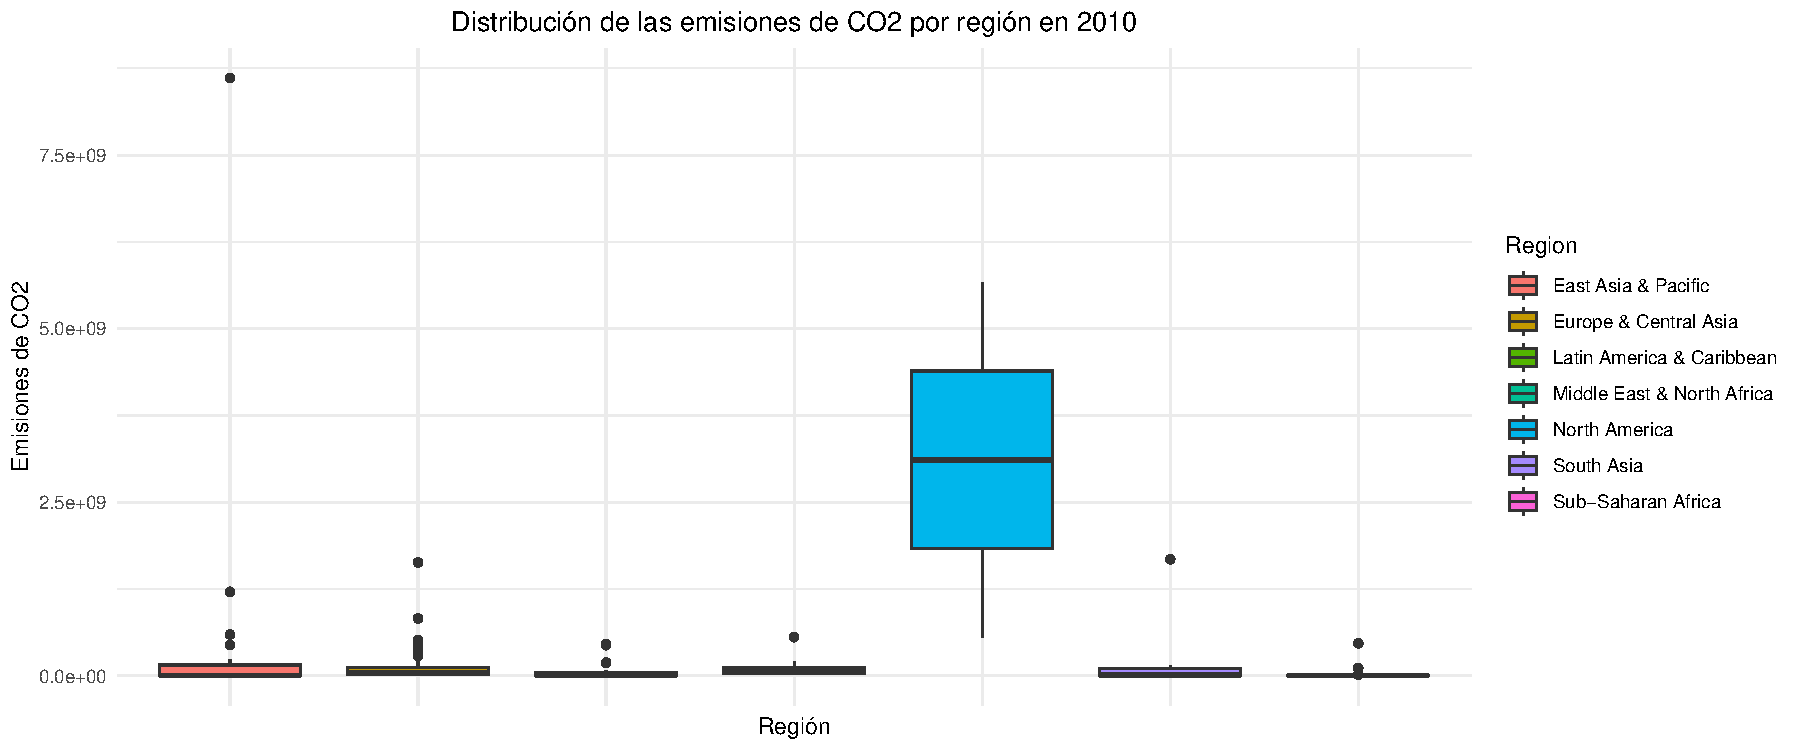
\includegraphics[keepaspectratio]{proyecto-Fabian_files/figure-latex/10-1.pdf}}
\caption{\label{fig:10}Distribución de emisiones por región}
\end{figure}

\begin{Shaded}
\begin{Highlighting}[]
\FunctionTok{ggplot}\NormalTok{(gdp\_joined\_data2[gdp\_joined\_data2}\SpecialCharTok{$}\NormalTok{Year }\SpecialCharTok{==} \DecValTok{2010}\NormalTok{,], }\FunctionTok{aes}\NormalTok{(}\AttributeTok{x =} \FunctionTok{factor}\NormalTok{(}\StringTok{\textasciigrave{}}\AttributeTok{Income group}\StringTok{\textasciigrave{}}\NormalTok{), }\AttributeTok{y =} \StringTok{\textasciigrave{}}\AttributeTok{Annual CO2 emissions}\StringTok{\textasciigrave{}}\NormalTok{, }\AttributeTok{fill =} \StringTok{\textasciigrave{}}\AttributeTok{Income group}\StringTok{\textasciigrave{}}\NormalTok{)) }\SpecialCharTok{+}
  \FunctionTok{geom\_boxplot}\NormalTok{() }\SpecialCharTok{+}
  \FunctionTok{labs}\NormalTok{(}
    \AttributeTok{x =} \StringTok{"Grupo Económico"}\NormalTok{,}
    \AttributeTok{y =} \StringTok{"Emisiones de CO2"}\NormalTok{,}
    \AttributeTok{title =} \StringTok{"Distribución de las emisiones de CO2 por grupo económico en 2010"}
\NormalTok{  ) }\SpecialCharTok{+}
  \FunctionTok{theme\_minimal}\NormalTok{() }\SpecialCharTok{+}
  \FunctionTok{theme}\NormalTok{(}
    \AttributeTok{axis.text.x =} \FunctionTok{element\_blank}\NormalTok{(),}
    \AttributeTok{axis.ticks.x =} \FunctionTok{element\_blank}\NormalTok{(),}
    \AttributeTok{plot.title =} \FunctionTok{element\_text}\NormalTok{(}\AttributeTok{hjust =} \FloatTok{0.5}\NormalTok{)}
\NormalTok{  )}
\end{Highlighting}
\end{Shaded}

\begin{figure}
\centering
\pandocbounded{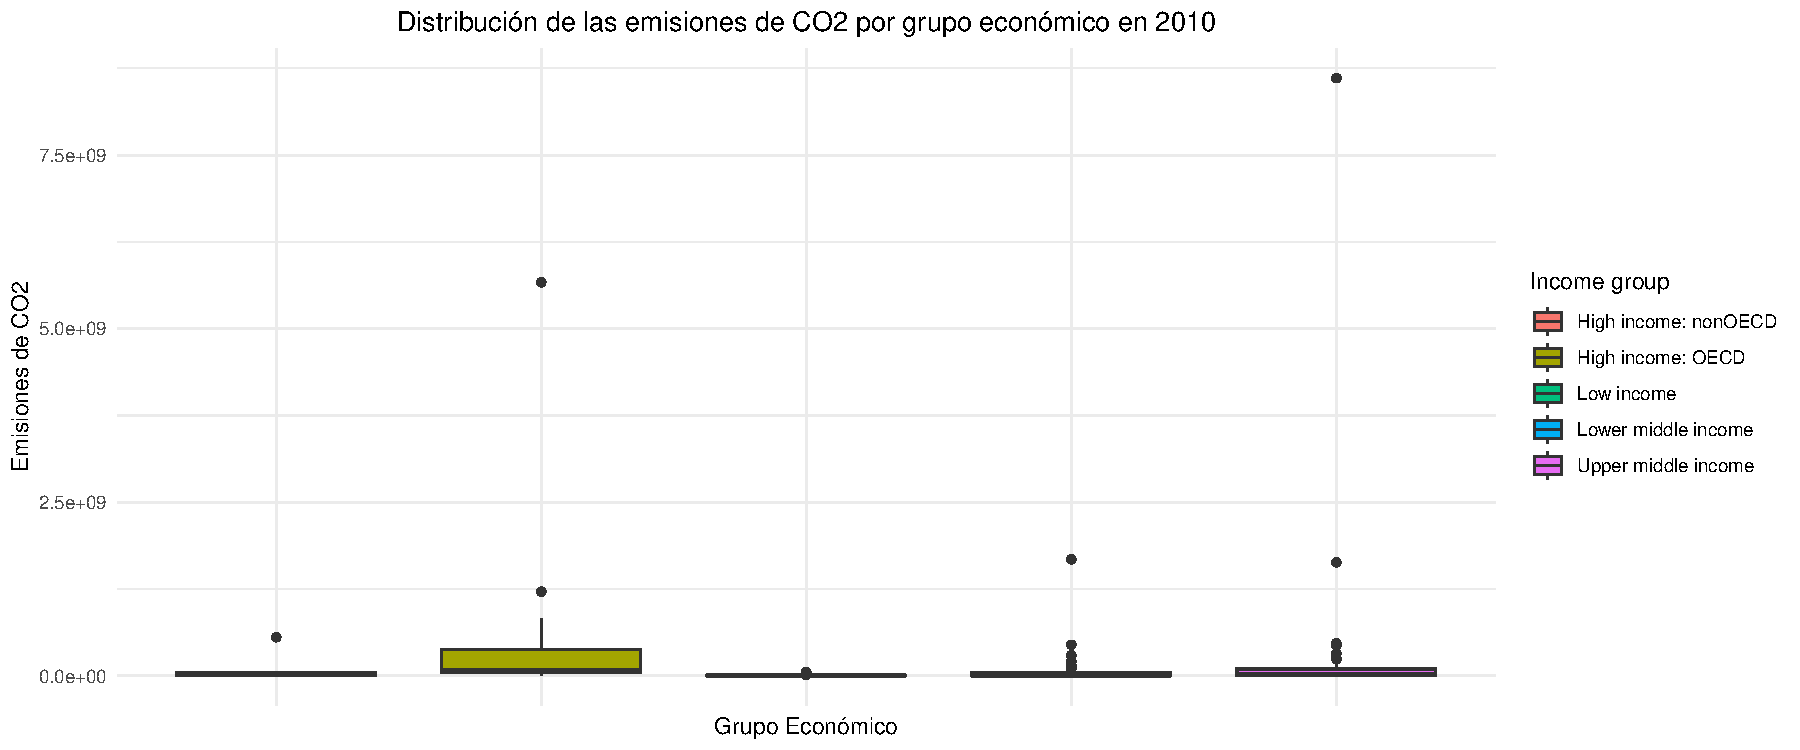
\includegraphics[keepaspectratio]{proyecto-Fabian_files/figure-latex/11-1.pdf}}
\caption{\label{fig:11}Distribución de emisiones por grupo económico}
\end{figure}

\section{Análisis de Proyecciones}\label{anuxe1lisis-de-proyecciones}

El conjunto de datos obtenido de \citep{ref155} nos provee proyecciones de cambio de temperatura y precipitaciones para cada país durante el perio 2045 a 2065. Esta información viene un campo de texto en formato `Bajo a Alto'. Para nuestro análisis, se extrajó ambos niveles para cada país y se promediaron, de forma que se obtuvo una proyección promedio de cambio de temperatura y precipitación para cada país.

\subsection{Proyección de cambio de temperatura}\label{proyecciuxf3n-de-cambio-de-temperatura}

Analizamos la proyección de cambio de temperatura, desagregada por ingreso y por región. El rango general de las proyecciones se sitúa entre aproximadamente 1.0 °C y 3.1 °C, con la mayoría de las medianas concentradas en torno a 2.2--2.5 °C, lo que indica que el calentamiento proyectado es un fenómeno de alcance global sin excepción regional significativa.

\begin{itemize}
\tightlist
\item
  Por región
\end{itemize}

Las diferencias por región son más pronunciadas. Asia Oriental y el Pacífico presenta la mediana más baja (\textasciitilde1.7 °C) y la distribución más comprimida, posiblemente asociada a efectos moderadores de la circulación oceánica en las zonas costeras e insulares de la región. En el extremo opuesto, Oriente Medio y África del Norte, América del Norte y Asia del Sur exhiben las medianas más elevadas (\textasciitilde2.5 °C), con cajas amplias que denotan variabilidad interna significativa entre países. África Subsahariana y Europa y Asia Central muestran medianas intermedias (\textasciitilde2.3 °C) pero con bigotes que se extienden hasta valores superiores a 3.0 °C, indicando que algunos países dentro de estas regiones podrían experimentar calentamientos considerablemente más severos. América Latina y el Caribe presenta la mayor dispersión interna de todas las regiones, con una caja que abarca desde aproximadamente 1.6 °C hasta 2.3 °C, coherente con la diversidad climática de un territorio que incluye desde zonas tropicales hasta regiones subpolares.

\begin{Shaded}
\begin{Highlighting}[]
\NormalTok{projected\_temperature\_change }\OtherTok{\textless{}{-}}\NormalTok{ climate\_change\_data }\SpecialCharTok{\%\textgreater{}\%} 
  \FunctionTok{filter}\NormalTok{(}\StringTok{\textasciigrave{}}\AttributeTok{Series code}\StringTok{\textasciigrave{}} \SpecialCharTok{==} \StringTok{"EN.CLC.PCAT.C"}\NormalTok{) }\SpecialCharTok{\%\textgreater{}\%} 
  \FunctionTok{select}\NormalTok{(}\StringTok{\textasciigrave{}}\AttributeTok{Country code}\StringTok{\textasciigrave{}}\NormalTok{, }\StringTok{\textasciigrave{}}\AttributeTok{Country name}\StringTok{\textasciigrave{}}\NormalTok{, }\StringTok{\textasciigrave{}}\AttributeTok{2011}\StringTok{\textasciigrave{}}\NormalTok{) }\SpecialCharTok{\%\textgreater{}\%} 
  \FunctionTok{mutate}\NormalTok{(}
    \AttributeTok{temp =} \FunctionTok{if\_else}\NormalTok{(}\FunctionTok{str\_detect}\NormalTok{(}\StringTok{\textasciigrave{}}\AttributeTok{2011}\StringTok{\textasciigrave{}}\NormalTok{, }\StringTok{" to "}\NormalTok{),}
                   \StringTok{\textasciigrave{}}\AttributeTok{2011}\StringTok{\textasciigrave{}}\NormalTok{,}
                   \ConstantTok{NA\_character\_}\NormalTok{)}
\NormalTok{  ) }\SpecialCharTok{\%\textgreater{}\%}
  \FunctionTok{separate}\NormalTok{(}
\NormalTok{    temp,}
    \AttributeTok{into =} \FunctionTok{c}\NormalTok{(}\StringTok{"Lowest"}\NormalTok{, }\StringTok{"Highest"}\NormalTok{),}
    \AttributeTok{sep =} \StringTok{" to "}
\NormalTok{  ) }\SpecialCharTok{\%\textgreater{}\%} 
  \FunctionTok{mutate}\NormalTok{(}
    \AttributeTok{Lowest =} \FunctionTok{as.numeric}\NormalTok{(Lowest),}
    \AttributeTok{Highest   =} \FunctionTok{as.numeric}\NormalTok{(Highest),}
    \AttributeTok{Mean    =} \FunctionTok{rowMeans}\NormalTok{(}\FunctionTok{cbind}\NormalTok{(Lowest, Highest), }\AttributeTok{na.rm =} \ConstantTok{TRUE}\NormalTok{)) }\SpecialCharTok{\%\textgreater{}\%}  
  \FunctionTok{select}\NormalTok{(}\SpecialCharTok{{-}}\StringTok{\textasciigrave{}}\AttributeTok{2011}\StringTok{\textasciigrave{}}\NormalTok{, }\SpecialCharTok{{-}}\NormalTok{Lowest, }\SpecialCharTok{{-}}\NormalTok{Highest)}

\NormalTok{projected\_precipitation\_change }\OtherTok{\textless{}{-}}\NormalTok{ climate\_change\_data }\SpecialCharTok{\%\textgreater{}\%} 
  \FunctionTok{filter}\NormalTok{(}\StringTok{\textasciigrave{}}\AttributeTok{Series code}\StringTok{\textasciigrave{}} \SpecialCharTok{==} \StringTok{"EN.CLC.PCPT.MM"}\NormalTok{) }\SpecialCharTok{\%\textgreater{}\%} 
  \FunctionTok{select}\NormalTok{(}\StringTok{\textasciigrave{}}\AttributeTok{Country code}\StringTok{\textasciigrave{}}\NormalTok{, }\StringTok{\textasciigrave{}}\AttributeTok{Country name}\StringTok{\textasciigrave{}}\NormalTok{, }\StringTok{\textasciigrave{}}\AttributeTok{2011}\StringTok{\textasciigrave{}}\NormalTok{) }\SpecialCharTok{\%\textgreater{}\%} 
  \FunctionTok{mutate}\NormalTok{(}
    \AttributeTok{temp =} \FunctionTok{if\_else}\NormalTok{(}\FunctionTok{str\_detect}\NormalTok{(}\StringTok{\textasciigrave{}}\AttributeTok{2011}\StringTok{\textasciigrave{}}\NormalTok{, }\StringTok{" to "}\NormalTok{),}
                   \StringTok{\textasciigrave{}}\AttributeTok{2011}\StringTok{\textasciigrave{}}\NormalTok{,}
                   \ConstantTok{NA\_character\_}\NormalTok{)}
\NormalTok{  ) }\SpecialCharTok{\%\textgreater{}\%}
  \FunctionTok{separate}\NormalTok{(}
\NormalTok{    temp,}
    \AttributeTok{into =} \FunctionTok{c}\NormalTok{(}\StringTok{"Lowest"}\NormalTok{, }\StringTok{"Highest"}\NormalTok{),}
    \AttributeTok{sep =} \StringTok{" to "}
\NormalTok{  ) }\SpecialCharTok{\%\textgreater{}\%} 
  \FunctionTok{mutate}\NormalTok{(}
    \AttributeTok{Lowest =} \FunctionTok{as.numeric}\NormalTok{(Lowest),}
    \AttributeTok{Highest   =} \FunctionTok{as.numeric}\NormalTok{(Highest),}
    \AttributeTok{Mean    =} \FunctionTok{rowMeans}\NormalTok{(}\FunctionTok{cbind}\NormalTok{(Lowest, Highest), }\AttributeTok{na.rm =} \ConstantTok{TRUE}\NormalTok{)) }\SpecialCharTok{\%\textgreater{}\%}  
  \FunctionTok{select}\NormalTok{(}\SpecialCharTok{{-}}\StringTok{\textasciigrave{}}\AttributeTok{2011}\StringTok{\textasciigrave{}}\NormalTok{, }\SpecialCharTok{{-}}\NormalTok{Lowest, }\SpecialCharTok{{-}}\NormalTok{Highest)}

\NormalTok{country\_data }\SpecialCharTok{\%\textgreater{}\%} 
  \FunctionTok{inner\_join}\NormalTok{(projected\_temperature\_change, }\AttributeTok{by=}\StringTok{"Country code"}\NormalTok{) }\SpecialCharTok{\%\textgreater{}\%} 
  \FunctionTok{select}\NormalTok{(}\SpecialCharTok{{-}}\StringTok{\textasciigrave{}}\AttributeTok{Country name.y}\StringTok{\textasciigrave{}}\NormalTok{, }\SpecialCharTok{{-}}\StringTok{\textasciigrave{}}\AttributeTok{Lending category}\StringTok{\textasciigrave{}}\NormalTok{) }\SpecialCharTok{\%\textgreater{}\%} 
  \FunctionTok{inner\_join}\NormalTok{(projected\_precipitation\_change, }\AttributeTok{by=}\StringTok{"Country code"}\NormalTok{) }\SpecialCharTok{\%\textgreater{}\%} 
  \FunctionTok{select}\NormalTok{(}\SpecialCharTok{{-}}\StringTok{\textasciigrave{}}\AttributeTok{Country name}\StringTok{\textasciigrave{}}\NormalTok{) }\SpecialCharTok{\%\textgreater{}\%} 
  \FunctionTok{drop\_na}\NormalTok{() }\SpecialCharTok{\%\textgreater{}\%} 
    \FunctionTok{rename}\NormalTok{(}
    \StringTok{\textasciigrave{}}\AttributeTok{Country Code}\StringTok{\textasciigrave{}} \OtherTok{=} \StringTok{\textasciigrave{}}\AttributeTok{Country code}\StringTok{\textasciigrave{}}\NormalTok{,}
    \StringTok{\textasciigrave{}}\AttributeTok{Temperature change}\StringTok{\textasciigrave{}} \OtherTok{=}\NormalTok{ Mean.x,}
    \StringTok{\textasciigrave{}}\AttributeTok{Precipitation change}\StringTok{\textasciigrave{}} \OtherTok{=}\NormalTok{ Mean.y}
\NormalTok{  ) }\OtherTok{{-}\textgreater{}}\NormalTok{ projected\_climate\_change\_country\_data}
\end{Highlighting}
\end{Shaded}

\begin{Shaded}
\begin{Highlighting}[]
\FunctionTok{ggplot}\NormalTok{(projected\_climate\_change\_country\_data, }\FunctionTok{aes}\NormalTok{(}\AttributeTok{x =} \FunctionTok{factor}\NormalTok{(}\StringTok{\textasciigrave{}}\AttributeTok{Region}\StringTok{\textasciigrave{}}\NormalTok{), }\AttributeTok{y =} \StringTok{\textasciigrave{}}\AttributeTok{Temperature change}\StringTok{\textasciigrave{}}\NormalTok{, }\AttributeTok{fill =} \StringTok{\textasciigrave{}}\AttributeTok{Region}\StringTok{\textasciigrave{}}\NormalTok{)) }\SpecialCharTok{+}
  \FunctionTok{geom\_boxplot}\NormalTok{() }\SpecialCharTok{+}
  \FunctionTok{labs}\NormalTok{(}
    \AttributeTok{x =} \StringTok{"Región"}\NormalTok{,}
    \AttributeTok{y =} \StringTok{"Cambio Proyectado de Temperatura Media (ºC)"}\NormalTok{,}
    \AttributeTok{title =} \StringTok{"Distribución del Cambio Proyectado de Temperatura Media (2045{-} 2065) por Región"}
\NormalTok{  ) }\SpecialCharTok{+}
  \FunctionTok{theme\_minimal}\NormalTok{() }\SpecialCharTok{+}
  \FunctionTok{theme}\NormalTok{(}
    \AttributeTok{axis.text.x =} \FunctionTok{element\_blank}\NormalTok{(),  }
    \AttributeTok{axis.ticks.x =} \FunctionTok{element\_blank}\NormalTok{(),}
    \AttributeTok{plot.title =} \FunctionTok{element\_text}\NormalTok{(}\AttributeTok{hjust =} \FloatTok{0.5}\NormalTok{) }
\NormalTok{  )}
\end{Highlighting}
\end{Shaded}

\begin{figure}
\centering
\pandocbounded{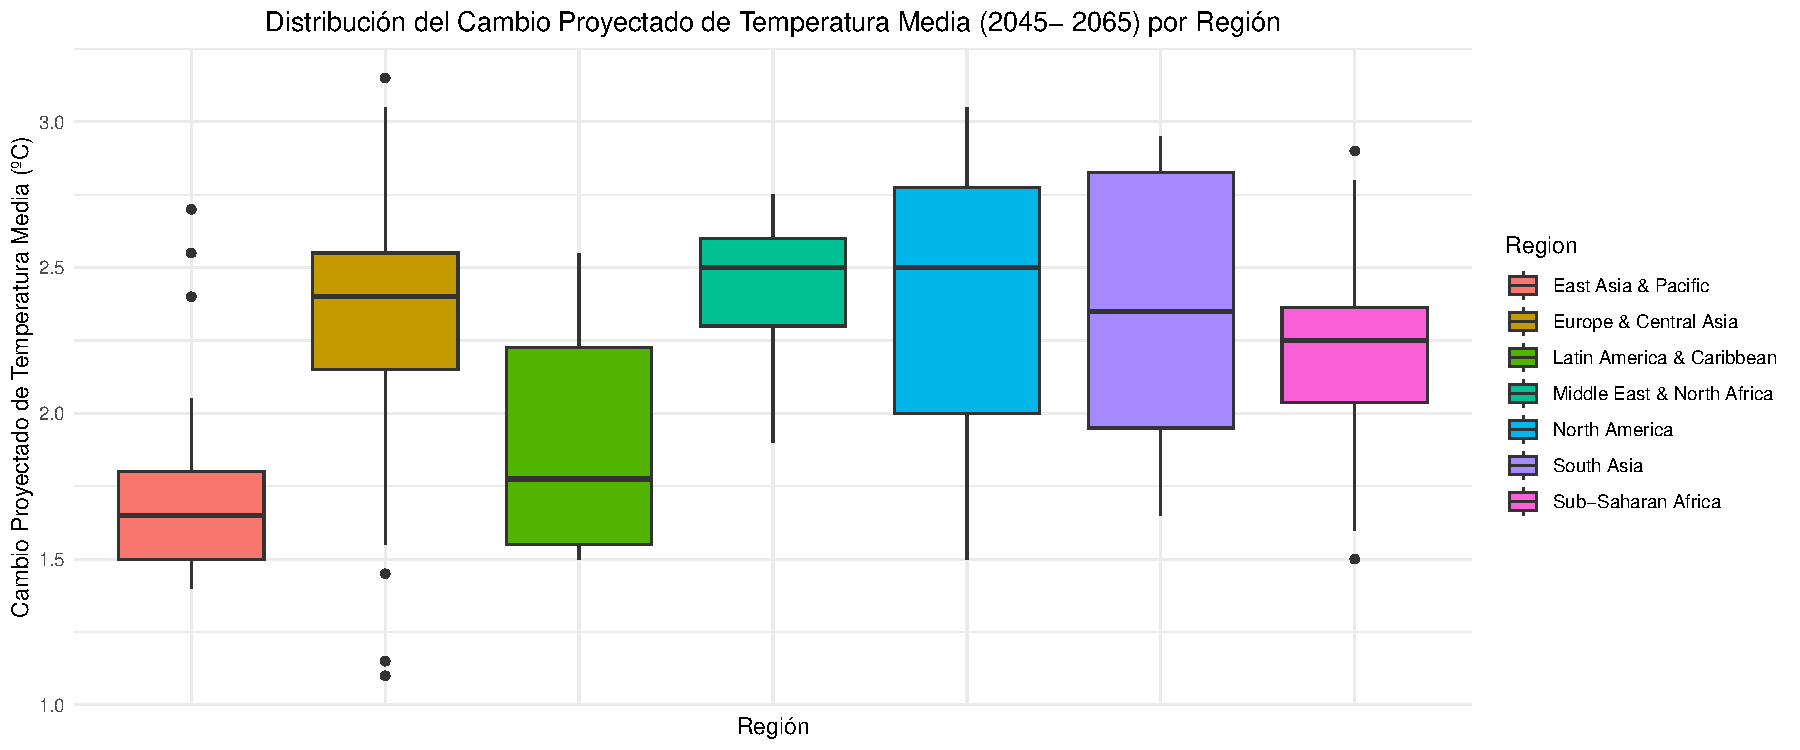
\includegraphics[keepaspectratio]{proyecto-Fabian_files/figure-latex/12-1.pdf}}
\caption{\label{fig:12}Proyección de cambio de temperatura por región}
\end{figure}

\begin{itemize}
\tightlist
\item
  Por Grupo Ecónomico
\end{itemize}

Las distribuciones por grupo económico son notablemente similares en sus medianas, oscilando entre 1.8 °C (alto ingreso no-OCDE) y 2.3 °C (bajo ingreso, ingreso medio-bajo e ingreso medio-alto). Sin embargo, la amplitud de las cajas intercuartílicas varía: los grupos de ingreso bajo e ingreso medio presentan mayor dispersión interna, reflejando la heterogeneidad geográfica de los países que los integran. El hallazgo analíticamente más relevante es la ausencia de una gradiente clara entre nivel de ingreso y magnitud del calentamiento proyectado: los países de bajo ingreso ---que históricamente han contribuido de forma marginal a las emisiones acumuladas--- enfrentarán incrementos de temperatura comparables o superiores a los de las economías que han sido responsables de la mayor parte de las emisiones históricas.

\begin{Shaded}
\begin{Highlighting}[]
\FunctionTok{ggplot}\NormalTok{(projected\_climate\_change\_country\_data, }\FunctionTok{aes}\NormalTok{(}\AttributeTok{x =} \FunctionTok{factor}\NormalTok{(}\StringTok{\textasciigrave{}}\AttributeTok{Income group}\StringTok{\textasciigrave{}}\NormalTok{), }\AttributeTok{y =} \StringTok{\textasciigrave{}}\AttributeTok{Temperature change}\StringTok{\textasciigrave{}}\NormalTok{, }\AttributeTok{fill =} \StringTok{\textasciigrave{}}\AttributeTok{Income group}\StringTok{\textasciigrave{}}\NormalTok{)) }\SpecialCharTok{+}
  \FunctionTok{geom\_boxplot}\NormalTok{() }\SpecialCharTok{+}
  \FunctionTok{labs}\NormalTok{(}
    \AttributeTok{x =} \StringTok{"Grupo Económico"}\NormalTok{,}
    \AttributeTok{y =} \StringTok{"Cambio Proyectado de Temperatura Media (ºC)"}\NormalTok{,}
    \AttributeTok{title =} \StringTok{"Distribución del Cambio Proyectado de Temperatura Media (2045{-} 2065) por Grupo Económico"}
\NormalTok{  ) }\SpecialCharTok{+}
  \FunctionTok{theme\_minimal}\NormalTok{() }\SpecialCharTok{+}
  \FunctionTok{theme}\NormalTok{(}
    \AttributeTok{axis.text.x =} \FunctionTok{element\_blank}\NormalTok{(),  }
    \AttributeTok{axis.ticks.x =} \FunctionTok{element\_blank}\NormalTok{(),}
    \AttributeTok{plot.title =} \FunctionTok{element\_text}\NormalTok{(}\AttributeTok{hjust =} \FloatTok{0.5}\NormalTok{) }
\NormalTok{  )}
\end{Highlighting}
\end{Shaded}

\pandocbounded{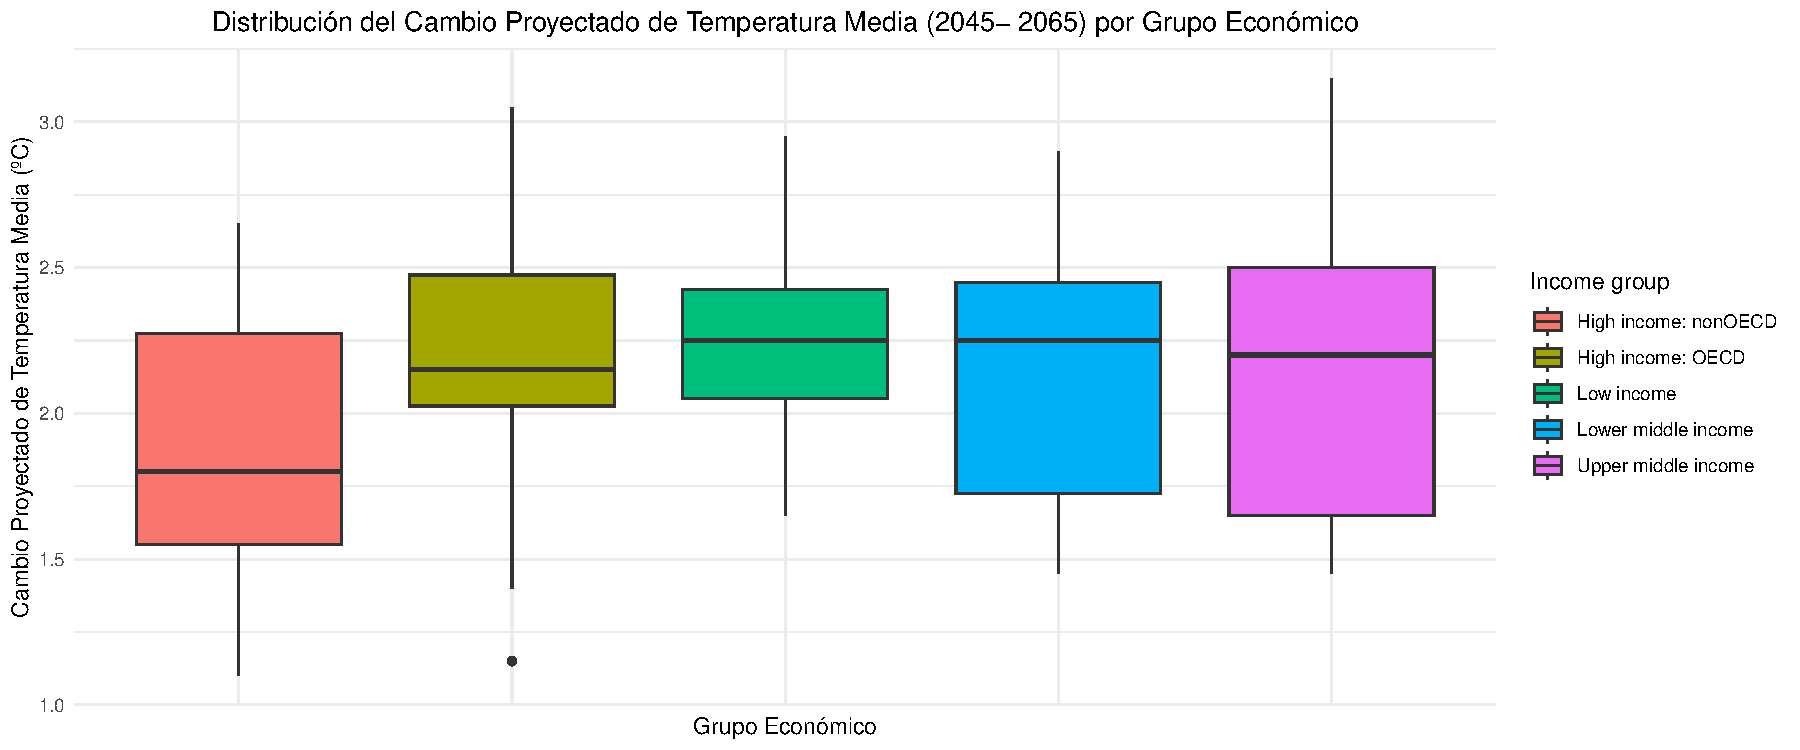
\includegraphics[keepaspectratio]{proyecto-Fabian_files/figure-latex/13-1.pdf}}
La lectura conjunta de ambos gráficos conduce a dos conclusiones de orden superior. Primero, el calentamiento proyectado es independiente del nivel de responsabilidad histórica en las emisiones: regiones de bajo ingreso y baja industrialización soportarán incrementos de temperatura equivalentes a los de las economías más emisoras, lo que refuerza el argumento de justicia climática en los marcos de negociación internacional. Segundo, la variabilidad intra-regional e intra-grupal es tan o más relevante que las diferencias entre categorías, sugiriendo que las políticas de adaptación climática deben diseñarse atendiendo a vulnerabilidades específicas de cada país, más que a clasificaciones de ingreso o región.

\subsection{Proyección de cambio en precipitaciones}\label{proyecciuxf3n-de-cambio-en-precipitaciones}

A diferencia de las proyecciones de temperatura ---donde todas las regiones convergen hacia incrementos positivos--- los gráficos de precipitación revelan una dinámica fundamentalmente distinta: el signo del cambio proyectado varía según la región, configurando un escenario en el que el calentamiento global produce simultáneamente exceso hídrico en algunas zonas y déficit severo en otras. Este patrón constituye uno de los impactos más complejos del cambio climático desde el punto de vista de la adaptación.

\begin{itemize}
\tightlist
\item
  Por Región
\end{itemize}

Por región, la heterogeneidad es marcada. Asia Oriental y el Pacífico presenta la mediana más alta (\textasciitilde+50 mm) y la mayor dispersión positiva, con outliers que superan los +300 mm, indicando que una fracción de sus países podría experimentar incrementos de precipitación muy significativos, probablemente asociados a la intensificación de sistemas oceánicos y ciclónicos. Asia del Sur y América del Norte también proyectan medianas positivas (\textasciitilde+50 mm y \textasciitilde+30 mm respectivamente), consistentes con el reforzamiento de regímenes de precipitación en latitudes medias y subtropicales húmedas. En contraste, América Latina y el Caribe, Europa y Asia Central, y especialmente Oriente Medio y África del Norte muestran medianas negativas o cercanas a cero, con cajas que se extienden predominantemente por debajo del eje, señalando tendencias hacia la aridización. África Subsahariana presenta una distribución centrada en torno a cero pero con alta dispersión en ambas direcciones, reflejando la coexistencia de zonas con incrementos y zonas con déficits dentro de una región geográficamente extensa y climáticamente diversa.

\begin{Shaded}
\begin{Highlighting}[]
\FunctionTok{ggplot}\NormalTok{(projected\_climate\_change\_country\_data, }\FunctionTok{aes}\NormalTok{(}\AttributeTok{x =} \FunctionTok{factor}\NormalTok{(}\StringTok{\textasciigrave{}}\AttributeTok{Region}\StringTok{\textasciigrave{}}\NormalTok{), }\AttributeTok{y =} \StringTok{\textasciigrave{}}\AttributeTok{Precipitation change}\StringTok{\textasciigrave{}}\NormalTok{, }\AttributeTok{fill =} \StringTok{\textasciigrave{}}\AttributeTok{Region}\StringTok{\textasciigrave{}}\NormalTok{)) }\SpecialCharTok{+}
  \FunctionTok{geom\_boxplot}\NormalTok{() }\SpecialCharTok{+}
  \FunctionTok{labs}\NormalTok{(}
    \AttributeTok{x =} \StringTok{"Región"}\NormalTok{,}
    \AttributeTok{y =} \StringTok{"Cambio Proyectado de Precipitación Promedio (mm)"}\NormalTok{,}
    \AttributeTok{title =} \StringTok{"Distribución del Cambio Proyectado de Precipitación Promedio (2045{-} 2065) por Región"}
\NormalTok{  ) }\SpecialCharTok{+}
  \FunctionTok{theme\_minimal}\NormalTok{() }\SpecialCharTok{+}
  \FunctionTok{theme}\NormalTok{(}
    \AttributeTok{axis.text.x =} \FunctionTok{element\_blank}\NormalTok{(),  }
    \AttributeTok{axis.ticks.x =} \FunctionTok{element\_blank}\NormalTok{(),}
    \AttributeTok{plot.title =} \FunctionTok{element\_text}\NormalTok{(}\AttributeTok{hjust =} \FloatTok{0.5}\NormalTok{)  }
\NormalTok{  )}
\end{Highlighting}
\end{Shaded}

\begin{figure}
\centering
\pandocbounded{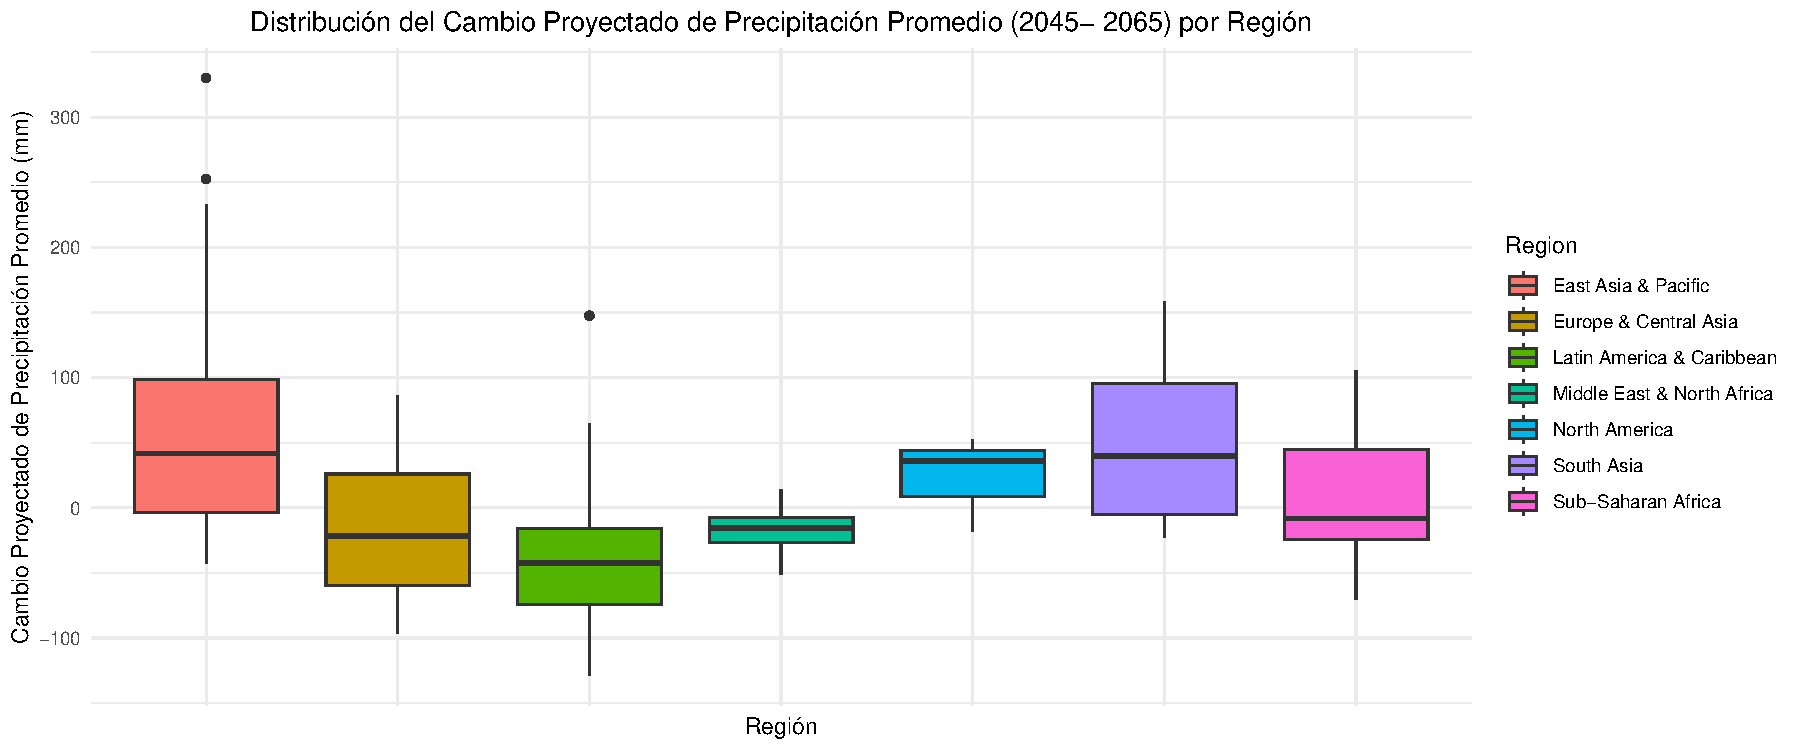
\includegraphics[keepaspectratio]{proyecto-Fabian_files/figure-latex/14-1.pdf}}
\caption{\label{fig:14}Proyección de cambio de precipitaciones por región}
\end{figure}

\begin{itemize}
\tightlist
\item
  Por grupo económico
\end{itemize}

Por grupo de ingreso, el patrón más relevante es que el grupo de alto ingreso no-OCDE presenta una mediana claramente negativa (\textasciitilde−40 mm), coherente con la concentración de países de este grupo en zonas geográficas áridas o semiáridas como el Golfo Pérsico y partes de Europa meridional. El grupo de alto ingreso OCDE muestra una mediana levemente positiva con dispersión moderada, mientras que los grupos de ingreso bajo e ingreso medio-bajo exhiben distribuciones más amplias con medianas próximas a cero, reflejando nuevamente la heterogeneidad geográfica de sus integrantes. Los outliers más extremos ---superando los +300 mm--- se concentran en los grupos de ingreso medio-bajo y medio-alto, correspondientes a países tropicales de gran extensión territorial.

\begin{Shaded}
\begin{Highlighting}[]
\FunctionTok{ggplot}\NormalTok{(projected\_climate\_change\_country\_data, }\FunctionTok{aes}\NormalTok{(}\AttributeTok{x =} \FunctionTok{factor}\NormalTok{(}\StringTok{\textasciigrave{}}\AttributeTok{Income group}\StringTok{\textasciigrave{}}\NormalTok{), }\AttributeTok{y =} \StringTok{\textasciigrave{}}\AttributeTok{Precipitation change}\StringTok{\textasciigrave{}}\NormalTok{, }\AttributeTok{fill =} \StringTok{\textasciigrave{}}\AttributeTok{Income group}\StringTok{\textasciigrave{}}\NormalTok{)) }\SpecialCharTok{+}
  \FunctionTok{geom\_boxplot}\NormalTok{() }\SpecialCharTok{+}
  \FunctionTok{labs}\NormalTok{(}
    \AttributeTok{x =} \StringTok{"Grupo Económico"}\NormalTok{,}
    \AttributeTok{y =} \StringTok{"Cambio Proyectado de Precipitación Promedio (mm)"}\NormalTok{,}
    \AttributeTok{title =} \StringTok{"Distribución del Cambio Proyectado de Precipitación Promedio (2045{-} 2065) por Grupo Económico"}
\NormalTok{  ) }\SpecialCharTok{+}
  \FunctionTok{theme\_minimal}\NormalTok{() }\SpecialCharTok{+}
  \FunctionTok{theme}\NormalTok{(}
    \AttributeTok{axis.text.x =} \FunctionTok{element\_blank}\NormalTok{(),   }
    \AttributeTok{axis.ticks.x =} \FunctionTok{element\_blank}\NormalTok{(),}
    \AttributeTok{plot.title =} \FunctionTok{element\_text}\NormalTok{(}\AttributeTok{hjust =} \FloatTok{0.5}\NormalTok{)   }
\NormalTok{  )}
\end{Highlighting}
\end{Shaded}

\pandocbounded{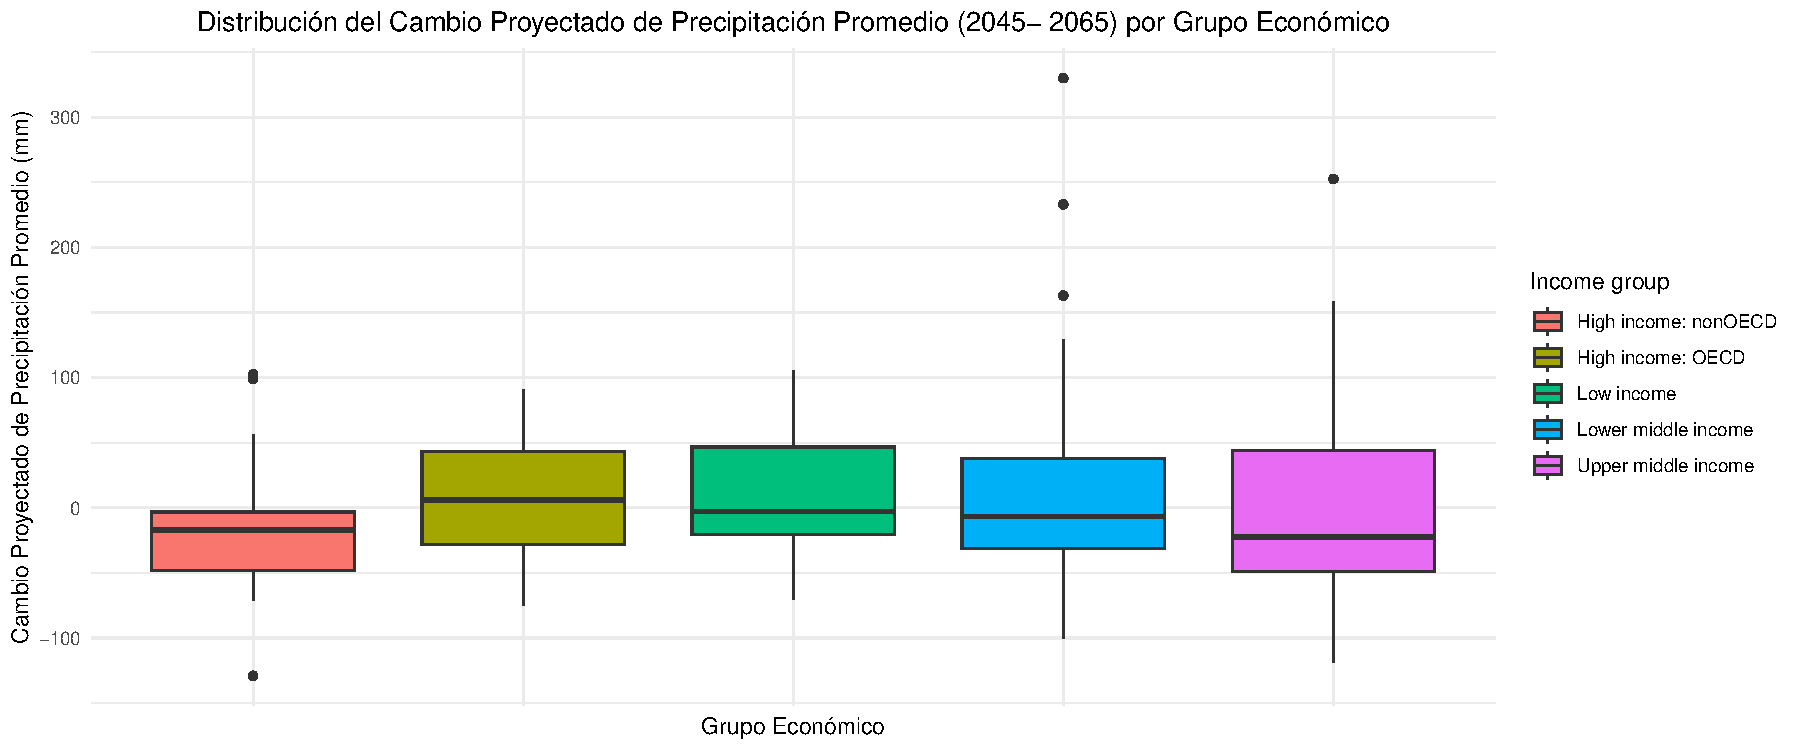
\includegraphics[keepaspectratio]{proyecto-Fabian_files/figure-latex/15-1.pdf}}
Las implicaciones analíticas de estos gráficos son significativas en dos dimensiones. Primero, la precipitación introduce una asimetría de impacto climático que la temperatura no captura: regiones que ya enfrentan estrés hídrico ---como Oriente Medio, partes de América Latina y el Mediterráneo--- verán agravada su situación, mientras que otras experimentarán riesgos asociados al exceso hídrico, como inundaciones e infraestructura desbordada. Segundo, y en articulación con los análisis previos, los países de menor ingreso que proyectan reducciones de precipitación enfrentan la combinación más adversa: mayor calentamiento relativo, menor capacidad adaptativa y potencial contracción de sus bases agrícolas, todo ello siendo responsables de una fracción ínfima de las emisiones históricas acumuladas que originan dichos impactos.

\chapter{Conclusiones}\label{conclusiones}

El conjunto de análisis presentados confirma una tendencia clara y sostenida: desde 1850, las emisiones globales de CO₂ y la temperatura media global han crecido de manera paralela y acelerada, con una correlación positiva que respalda la relación entre actividad industrial humana y calentamiento global. A escala regional, se evidencia que la industrialización y el crecimiento económico son los principales motores del aumento de emisiones. Las economías más desarrolladas muestran señales de separación gradual entre crecimiento y emisiones, mientras que Asia Oriental concentra los mayores incrementos del período 1990--2010, impulsados por una expansión industrial con alta dependencia de combustibles fósiles.

Sin embargo, el hallazgo más importante es la profunda desigualdad entre quiénes han causado el problema y quiénes sufrirán sus peores consecuencias. Los países de menor ingreso ---que han contribuido muy poco a las emisiones históricas--- enfrentarán aumentos de temperatura similares a los de las economías más contaminantes y, en muchos casos, reducciones de lluvia que pondrán en riesgo su agricultura y su acceso al agua. Apoyar la adaptación de estos países no es un asunto secundario, sino una parte esencial de cualquier respuesta climática global que quiera ser justa y efectiva.

  \bibliography{book.bib,packages.bib}

\end{document}
